% !TeX root = ..\main.tex

\section{Kiến trúc hệ thống}
\subsection{Lựa chọn kiến trúc}
 
\hspace*{0.5cm}Để chọn lựa kiến trúc phù hợp với hệ thống, chúng ta xem xét ưu điểm và nhược điểm của từng loại kiến trúc.\\
 
\begin{table}[h]
    \begin{tabular}{|p{3cm}|p{12cm}|}
        \hline
        \textbf{Tên kiến trúc} & Layer\\
        \hline
        \textbf{Mô tả}         & Kiến trúc được xây dựng thành nhiều lớp, các thành phần trong cùng một lớp có cùng nhiệm vụ với nhau; mỗi lớp sẽ cung cấp dịch vụ cho tầng trên của nó \\
        \hline
        \textbf{Ưu điểm}       & Có bản chất là hệ thống nguyên khối nên đơn giản, dễ xây dựng, chi phí thấp khi xây dựng bảo trì đồng thời có thể tăng tính tin cậy dựa vào số lượng các lớp \\
        \hline
        \textbf{Nhược điểm}    & Khả năng co giản, mở rộng thấp; hiệu xuất thấp vì không thể xử lý các tác vụ song song; khả năng chịu lỗi kém\\
        \hline
        \textbf{Sử dụng cho}   & Sử dụng trong các hệ thống nhỏ, không yêu cầu hiệu năng cao; các hệ thống được xây dựng trên một hệ thống có sẵn trước đó \\
        \hline
    \end{tabular}
    \caption{Kiến trúc Layer}
\end{table}
 
\begin{table}[h]
    \begin{tabular}{|p{3cm}|p{12cm}|}
        \hline
        \textbf{Tên kiến trúc} & Service-Based\\
        \hline
        \textbf{Mô tả}         & Kiến trúc được xây dựng thành các lớp phân tán, sử dụng các dịch vụ web kết nối tới một cơ sở dữ liệu nguyên khối     \\
        \hline
        \textbf{Ưu điểm}       & Sử dụng chung một cơ sở dữ liệu nên độ tin cậy, tính nhất quán dữ liệu cao; khả năng chịu lỗi tốt \\
        \hline
        \textbf{Nhược điểm}    & Sử dụng một cơ sở dữ liệu duy nhất nên khả năng co giãn mở rộng không linh hoạt   \\
        \hline
        \textbf{Sử dụng cho}   & Phù hợp với các hệ thống không quá lớn, các hệ thống phân chia thành từng domain                   \\
        \hline
    \end{tabular}
    \caption{Kiến trúc Service-based}
\end{table}
 
\begin{table}[h]
    \begin{tabular}{|p{3cm}|p{12cm}|}
        \hline
        \textbf{Tên kiến trúc} & Microservices\\
        \hline
        \textbf{Mô tả}         & Kiến trúc phân tán được xây dựng dựa trên điều phối các dịch vụ web tách biệt, hoạt động độc lập hoàn toàn các thành phần bao gồm cả cơ sở dữ liệu    \\
        \hline
        \textbf{Ưu điểm}       & Xây dựng dựa trên các dịch vụ web độc lập hoàn toàn nên khả năng co giãn, mở rộng cao; khả năng chịu lỗi tốt; dễ dàng thay đổi\\
        \hline
        \textbf{Nhược điểm}    & Các dịch vụ web phải giao tiếp nhiều do đó hiệu xuất không được đảm bảo; xây dựng khó khăn và chi phí lớn; khó duy trì tính nhất quán dữ liệu \\
        \hline
        \textbf{Sử dụng cho}   & Phù hợp với các hệ thống lớn, yêu cầu khả năng mở rộng cao trong tương lai                  \\
        \hline
    \end{tabular}
    \caption{Kiến trúc Microservices}
\end{table}
 
\newpage
 
\begin{table}[h]
    \begin{tabular}{|p{3cm}|p{12cm}|}
        \hline
        \textbf{Tên kiến trúc} & Event-Driven\\
        \hline
        \textbf{Mô tả}         & Kiến trúc không đồng bộ phân tán được xây dựng dựa trên các thành phần xử lý sự kiện không đồng bộ tách rời nhau \\
        \hline
        \textbf{Ưu điểm}       & Hiệu năng cao do thực hiện các tác vụ bất đồng bộ tách rời; khả năng mở rộng cao; khả năng chịu lỗi tốt \\
        \hline
        \textbf{Nhược điểm}    & Khó xây dựng và khó kiểm thử \\
        \hline
        \textbf{Sử dụng cho}   & Phù hợp với các hệ thống yêu cầu hiệu năng cao \\
        \hline
    \end{tabular}
    \caption{Kiến trúc Event-Driven}
\end{table}
 
 
Từ những thông tin trên, để phù hợp với hệ thống có khả năng mở rộng, thay đổi cao nhóm chọn kiến trúc Microservices. Bên cạnh đó nhóm sẽ kết hợp với kiến trúc Event-Driven để đảm bảo hiệu năng của hệ thống đối với các tác vụ bất đồng bộ

\subsection{Tổng quan kiến trúc}
 
\begin{figure}[!htp]
    \centering
    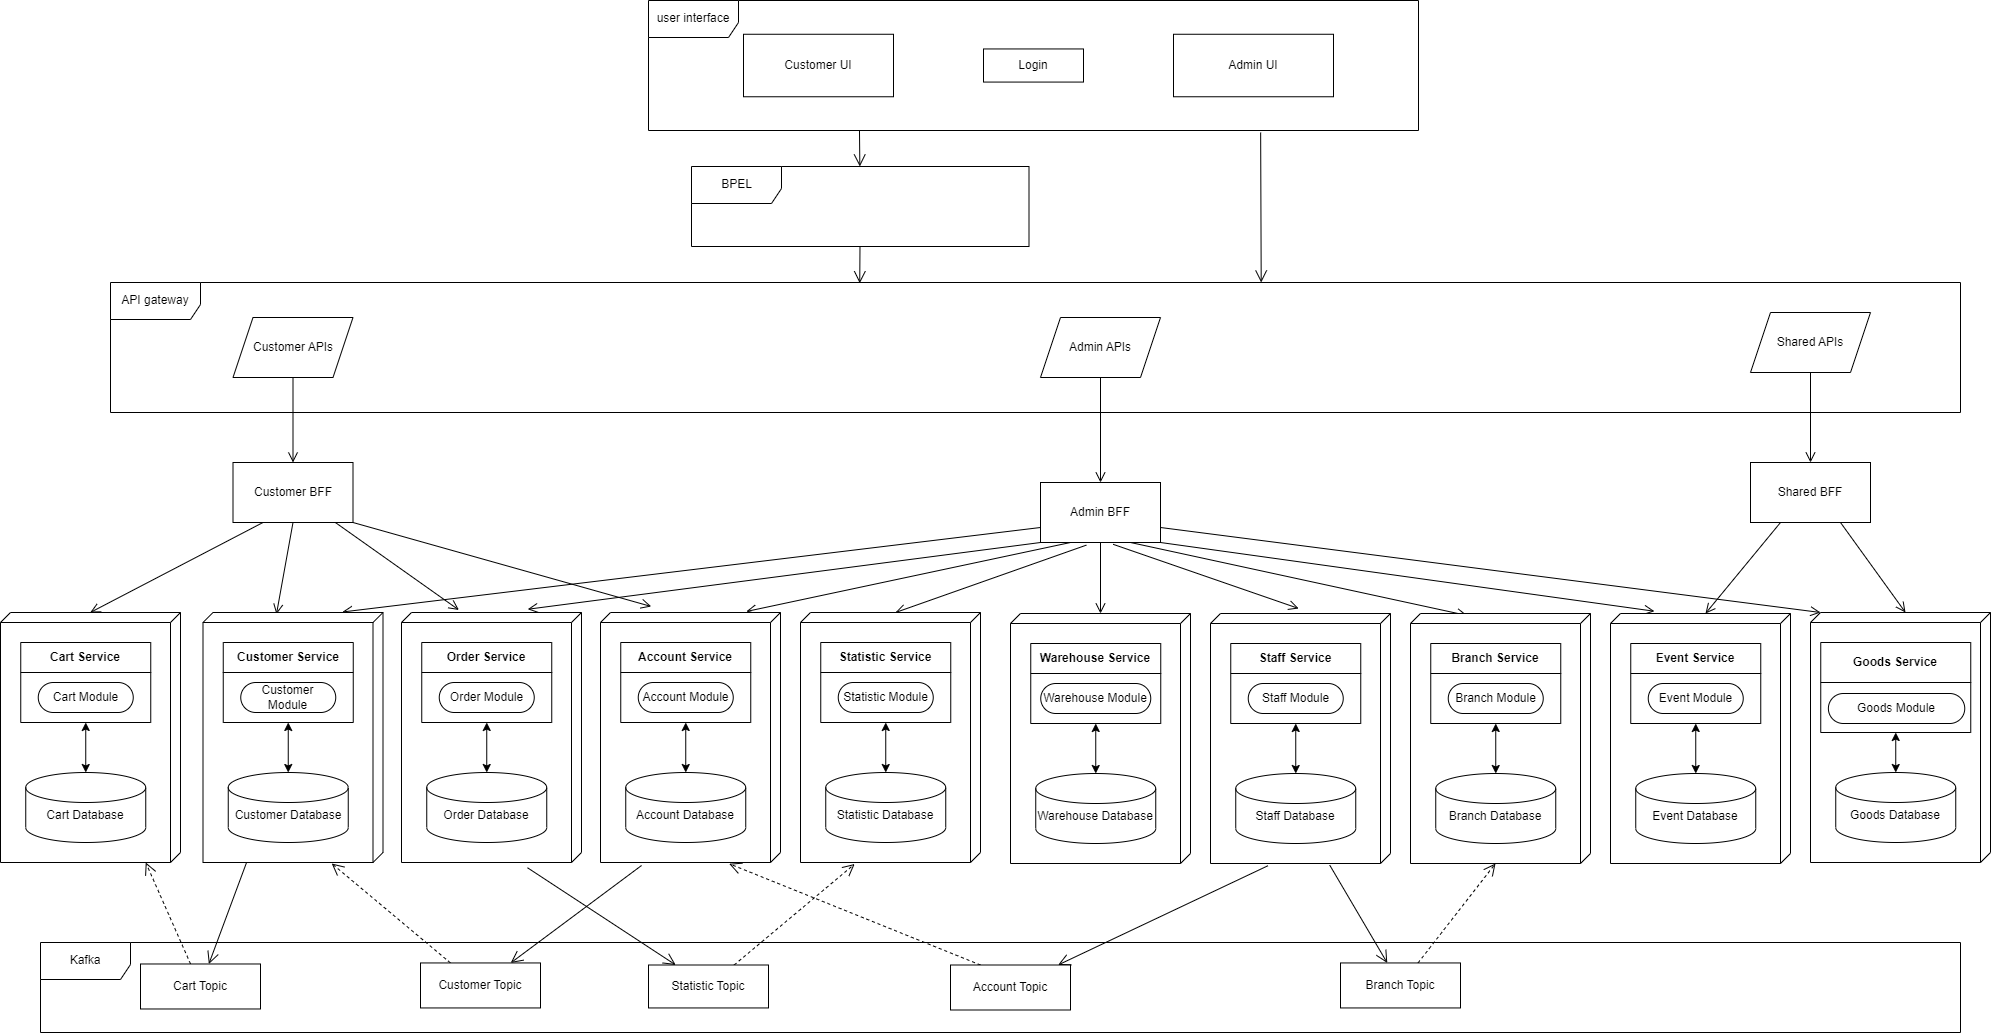
\includegraphics[width=6in]{img/Architecture/general-architect.png}
    \newline
    \caption{Tổng quan kiến trúc hệ thống}
\end{figure}
 
Hệ thống được xây dựng dựa trên kiến Microservice và được chia thành nhiều tầng:
\begin{itemize}
    \item Tầng User Interface: Tầng giao diện tương tác với người dùng
    \item Tầng BPEL: Tầng xây dựng quy trình BPEL, điều phối các quy trình nghiệp vụ trong hệ thống
    \item Tầng API Gateway: Tầng xuất các Api từ các dịch vụ web đưa đến quy trình BPEL
    \item Tầng BFF: Đóng vai trò trong việc kiểm tra các hoạt động trung gian khi nhận yêu cầu từ phía người dùng
    \item Tầng Web Service: Bao gồm các dịch vụ web
\end{itemize}
 
Bên cạnh các thành phần trên, để hiện thực việc giao tiếp bất đồng bộ giữa các dịch vụ web, hệ thống sử dụng Kafka. Đây là một hàng đợi thông điệp pub/sub dùng để lưu trữ và gửi đi các thông điệp.
Ta có thể tạo nên các \textbf{topic} trong Kafka. Các dịch vụ web có thể publish thông điệp lên một hoặc nhiều topic,
và khi một dịch vụ web subscribe vào một topic, nó có thể nhận dữ liệu từ topic đó.
Khi một thông điệp được gửi lên từ một dịch vụ Web, thông điệp sẽ được lưu trong hàng đợi thông điệp.
Những dịch vụ web subscribe vào topic này sau đó sẽ nhận được thông điệp này để xử lý.
Khi việc xử lý thất bại, bao gồm cả việc gửi thông điệp đến các subscriber thất bại, chúng ta có thể gửi lại thông điệp đó.
Vì điểm mạnh về multiple-sub và multiple-pub (một dịch vụ web có thể publish lên nhiều topic, cũng như có thể subscribe vào nhiều topic), cùng với việc hỗ trợ retry khi xảy ra lỗi, mà Kafka được nhóm lựa chọn sử dụng trong hệ thống.
 
\par Trong hệ thống, nhóm tổ chức các topic theo nhu cầu gửi thông điệp bất đồng bộ đến các dịch vụ web đích. Theo cách tổ chức này, một topic sẽ chỉ được subscribe bởi một dịch vụ web, và đó là dịch vụ web đích nhận và xử lý thông điệp. Trong khi đó, có thể có nhiều dịch vụ web subscribe vào một topic, tùy theo nhu cầu của các dịch vụ web.


\subsection{Tầng User Interface}
\subsubsection{CustomerUI}
Module này bao gồm các class dùng để hiển thị UI đối với phía khách hàng
\begin{figure}[!htp]
    \centering
    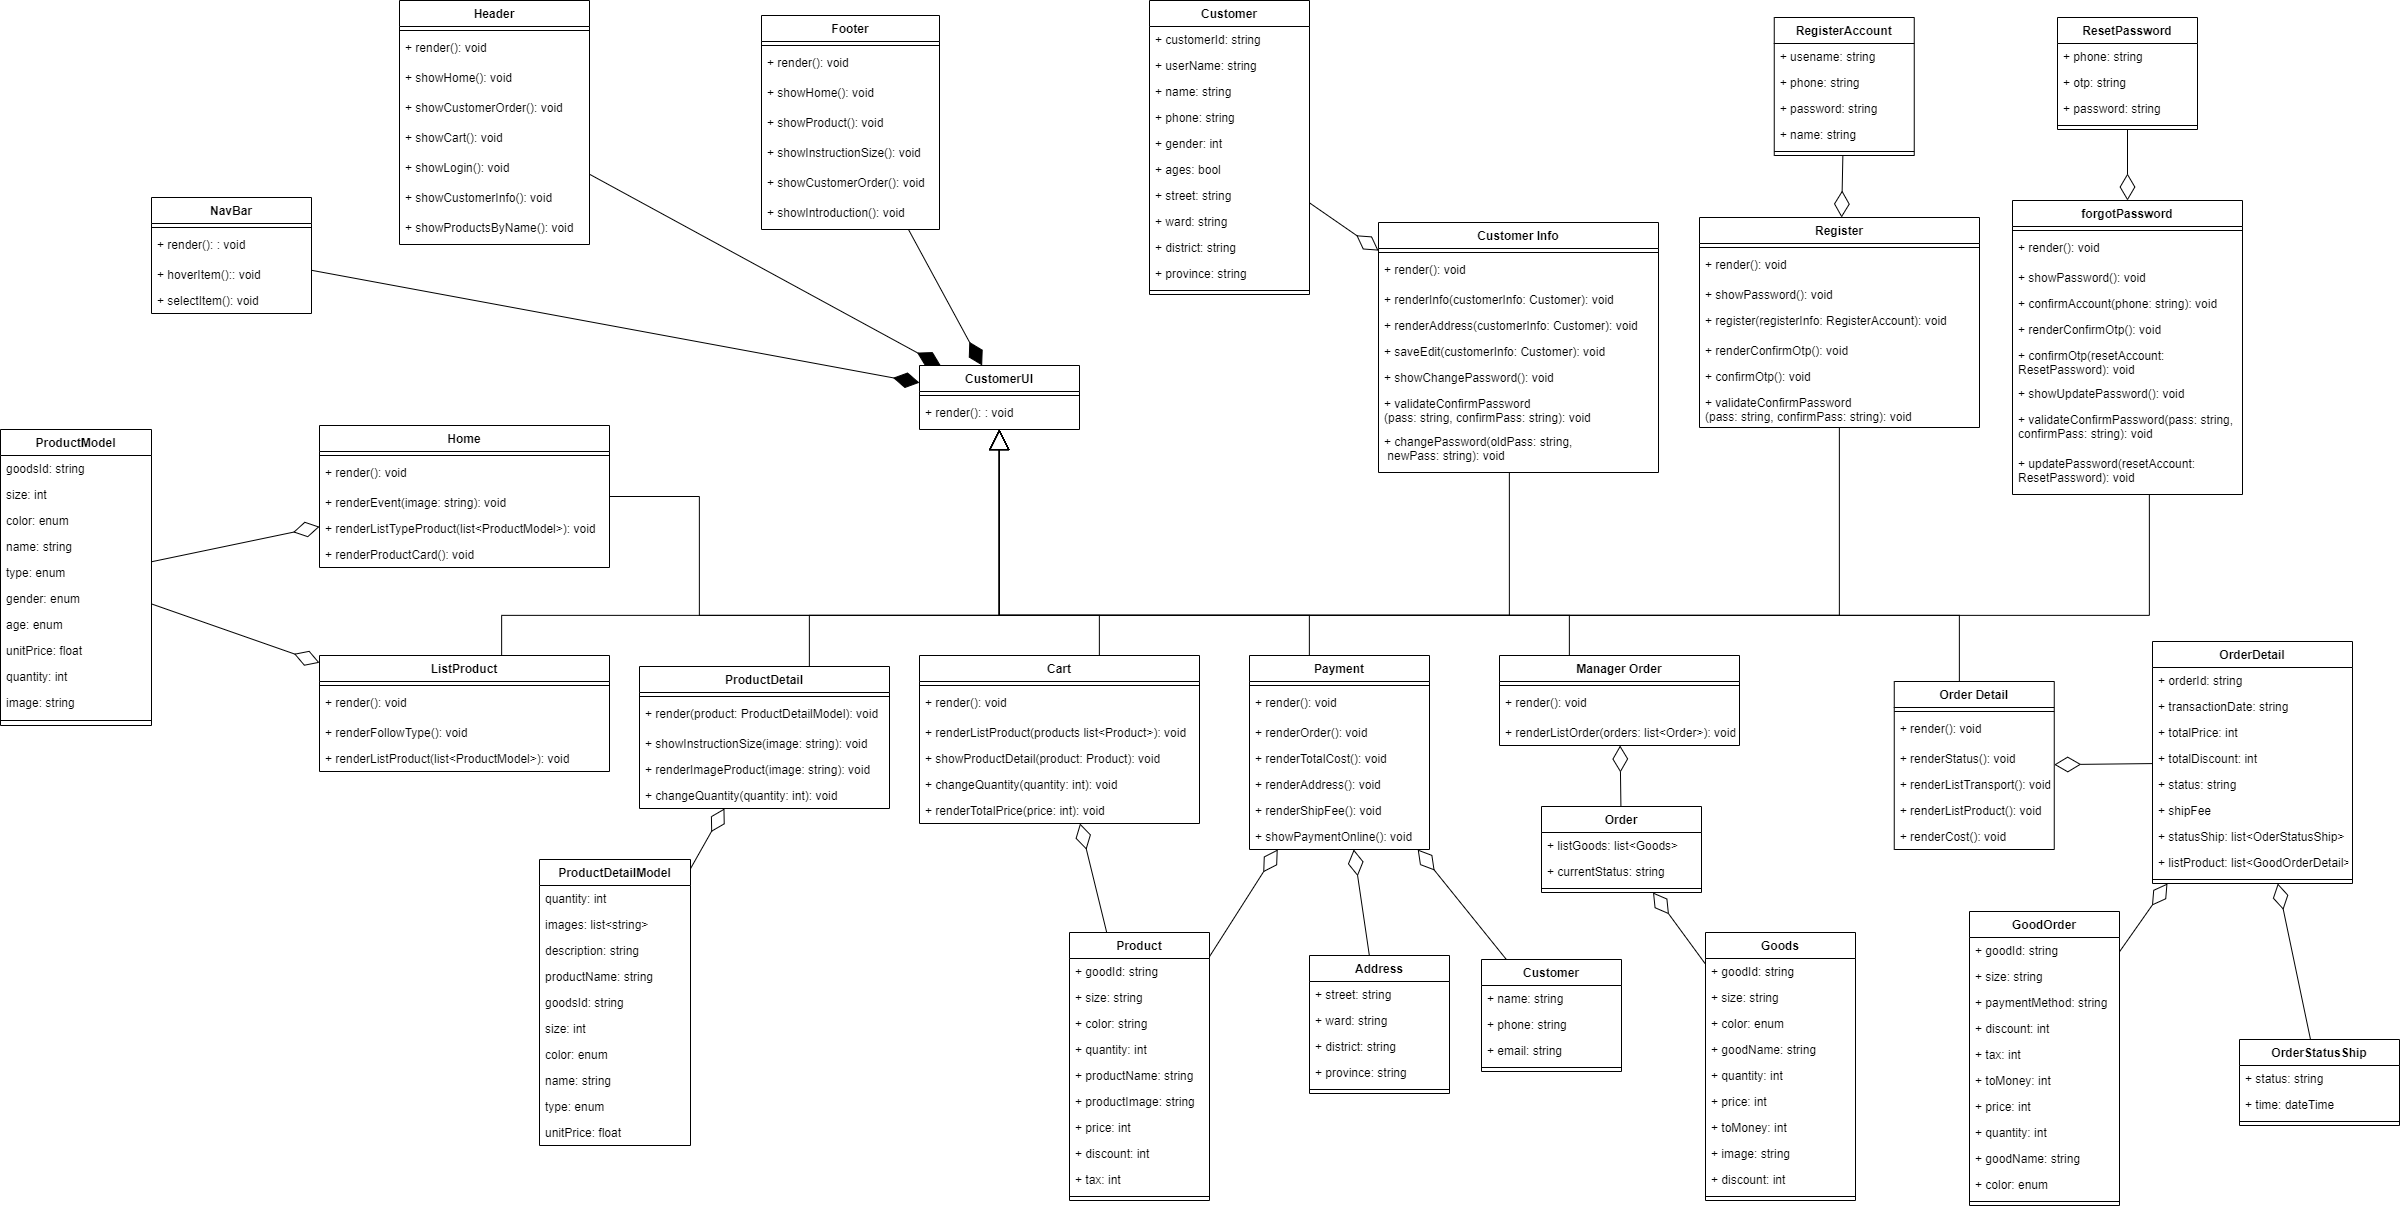
\includegraphics[width=17cm]{img/Architecture/UI/customer UI.png}
    \newline
    \caption{Lược đồ class của Module CustomerUI}
\end{figure}
 
\begin{quote}
 
    \subsubsubsection*{CustomerUI}
    Giao diện chính của khách hàng khi truy cập vào trang web của hệ thống.\\
    Phương thức:
    \begin{itemize}
        \item render(): Hiển thị lên màn hình của khách hàng.
    \end{itemize}
   
    \subsubsubsection*{NavBar}
    Thành phần luôn có của giao diện của khách hàng hiển thị các lựa chọn truy cập nhanh cho khách hàng.\\
    Phương thức:
    \begin{itemize}
        \item render(): Hiển thị lên màn hình của khách hàng.
        \item hoverItem(): Hiển thị lên màn hình giao diện các lựa chọn khi người dùng rê chuột đến các thể loại ở thanh navbar.
        \item selectItem(): Hiển thị lên màn hình giao diện tương ứng với lựa chọn của khách hàng trên thanh navbar.
    \end{itemize}
   
    \subsubsubsection*{Header}
    Thành phần luôn có của giao diện của khách hàng hiển thị các thông tin về tài khoản của khách hàng cũng như logo và chức năng tìm kiếm cho khách hàng.\\
    Phương thức:
    \begin{itemize}
        \item render(): Hiển thị lên màn hình của khách hàng.
        \item showHome(): Hiển thị về trang chủ mặc định của hệ thống.
        \item showCustomerOrder(): Hiển thị lên màn hình danh sách đơn hàng của khách hàng khi đã đăng nhập.
        \item showCart(): Hiển thị lên màn hình thông tin giỏ hàng của khách hàng khi đã đăng nhập.
        \item showLogin(): Hiển thị lên màn hình trang đăng nhập cho khách hàng khi chưa đăng nhập.
        \item showCustomerInfo(): Hiển thị lên màn hình thông tin chi tiết tài khoản của khách hàng khi đã đăng nhập.
        \item showProductByName(): Hiển thị lên màn hình danh sách các sản phẩm khi người dùng chọn tìm kiếm.
    \end{itemize}
   
    \subsubsubsection*{Footer}
    Thành phần luôn có của giao diện của khách hàng hiển thị các thông tin về hệ thống.\\
    Phương thức:
    \begin{itemize}
        \item render(): Hiển thị lên màn hình của khách hàng.
        \item showHome(): Hiển thị về trang chủ mặc định của hệ thống.
        \item showProduct(): Hiển thị lên màn hình danh sách tất cả sản phẩm của hệ thống.
        \item showInstructionSize(): Hiển thị lên màn hình thông tin hướng dẫn chọn size.
        \item showCustomerOrder(): Hiển thị lên màn hình trang danh sách các đơn hàng của khách hàng khi đã đăng nhập.
        \item showIntroduction(): Hiển thị lên màn hình trang giới thiệu về hệ thống cửa hàng.
    \end{itemize}
   
    \subsubsubsection*{Home}
    Màn hình mặc định của người dùng sau khi truy cập vào trang web của hệ thống.\\
    Phương thức:
    \begin{itemize}
        \item render(): Hiển thị lên màn hình của khách hàng.
        \item renderEvent(): Hiển thị thông tin các sự kiện đang diễn ra.
        \item renderListTypeProduct(): Hiển thị danh sách các sản phẩm nổi bật theo từng thể loại.
    \end{itemize}
   
    \subsubsubsection*{ListProduct}
    Màn hình hiển thị danh sách tất cả sản phẩm của hệ thống cho khách hàng.\\
    Phương thức:
    \begin{itemize}
        \item render(): Hiển thị lên màn hình của khách hàng.
        \item renderFollowType(): Hiển thị danh sách sản phẩm theo đặc điểm và thể loại.
        \item renderListProduct(): Hiển thị danh sách các sản phẩm.
    \end{itemize}
   
    \subsubsubsection*{ProductDetail} Màn hình hiển thị danh sách tất cả sản phẩm của hệ thống cho khách hàng.\\
    Phương thức:
    \begin{itemize}
        \item render(): Hiển thị lên màn hình của khách hàng.
        \item showInstructionSize(): Hiển thị lên màn hình thông tin hướng dẫn chọn size.
        \item renderImageProduct(): Hiển thị hình ảnh sản phẩm mà khách hàng chọn.
        \item changeQuantity(): Thay đổi số lượng sản phẩm để thêm vào giỏ hàng.
    \end{itemize}
   
    \subsubsubsection*{Cart}
    Màn hình hiển thị thông tin giỏ hàng của khách hàng.\\
    Phương thức:
    \begin{itemize}
        \item render(): Hiển thị lên màn hình của khách hàng.
        \item renderListProduct(): Hiển thị danh sách sản phẩm có trong giỏ hàng.
        \item showProductDetail(): Chuyển đến trang thông tin chi tiết của sản phẩm.
        \item changeQuantity(): Thay đổi số lượng sản phẩm trong giỏ hàng.
        \item renderTotalPrice(): Hiển thị tổng giá tiền của các sản phẩm được chọn trong giỏ hàng.
    \end{itemize}
   
    \subsubsubsection*{Payment}
    Màn hình hiển thị trang thanh toán cho khách hàng.\\
    Phương thức:
    \begin{itemize}
        \item render(): Hiển thị lên màn hình của khách hàng.
        \item renderOrder(): Hiển thị đơn hàng.
        \item renderTotalCost(): Hiển thị toàn bộ chi phí đơn hàng.
        \item renderAddress(): Hiển thị địa chỉ đơn hàng.
        \item renderShipFee(): Hiển thị giá tiền vận chuyển đơn hàng.
        \item ShowPaymentOnline(): Hiển thị màn hình thanh toán online.
    \end{itemize}
   
    \subsubsubsection*{ Manager Order}
    Màn hình hiển thị danh sách các đơn hàng của khách hàng.\\
    Phương thức:
    \begin{itemize}
        \item render(): Hiển thị lên màn hình của khách hàng.
        \item renderListOrder(): Hiển thị danh sách đơn hàng.
        \item showOrderDetail(): Hiển thị thông tin chi tiết của đơn hàng.
    \end{itemize}
   
    \subsubsubsection*{Order Detail}
    Màn hình hiển thị thông tin chi tiết đơn hàng của khách hàng.\\
    Phương thức:
    \begin{itemize}
        \item render(): Hiển thị lên màn hình của khách hàng.
        \item renderStatus(): Hiển thị trạng thái của đơn hàng.
        \item renderListTransport(): Hiển thị danh sách thông tin quá trình vận chuyển.
        \item renderListProduct(): Hiển thị danh sách sản phẩm có trong đơn hàng.
        \item renderCost(): Hiển thị danh sách các khoản chi phí của đơn hàng.
    \end{itemize}
   
    \subsubsubsection*{Forgot Password}
    Màn hình hiển thị trang tạo lại mật khẩu cho tài khoản của khách hàng.\\
    Phương thức:
    \begin{itemize}
        \item render(): Hiển thị lên màn hình của khách hàng.
        \item showPassword(): Hiển thị mật khẩu khỏi trạng thái bị ẩn.
        \item confirmAccount(): Xác nhận tài khoản muốn đổi mật khẩu.
        \item renderConfirmOtp(): Hiển thị màn hình xác nhận mã OTP.
        \item confirmOtp(): Gửi xác nhận mã OTP.
        \item showUpdatePassword(): Hiển thị trang cập nhật mật khẩu mới cho tài khoản.
        \item validateConfirmPassword(): Kiểm tra thông tin nhập lại mật khẩu của khách hàng.
        \item updatePassword(): Gửi thông tin cập nhật mật khẩu mới cho tài khoản.
    \end{itemize}
   
    \subsubsubsection*{Register}
    Màn hình hiển thị trang đăng ký tài khoản cho khách hàng.\\
    Phương thức:
    \begin{itemize}
        \item render(): Hiển thị lên màn hình của khách hàng.
        \item showPassword(): Hiển thị mật khẩu khỏi trạng thái bị ẩn.
        \item register(): gửi thông tin xác nhận.
        \item renderConfirmOtp(): Hiển thị màn hình xác nhận mã OTP.
        \item confirmOtp(): Gửi xác nhận mã OTP.
        \item validateConfirmPassword(): Kiểm tra thông tin nhập lại mật khẩu của khách hàng.
    \end{itemize}
   
    \subsubsubsection*{Customer Info}
    Màn hình hiển thị trang thông tin chi tiết tài khoản của khách hàng.\\
    Phương thức:
    \begin{itemize}
        \item render(): Hiển thị lên màn hình của khách hàng.
        \item renderInfo(): Hiển thị thông tin chung của khách hàng.
        \item renderAddress(): Hiển thị thông tin địa chỉ các khách hàng.
        \item saveEdit(): gửi đi thông tin tài khoản đã chỉnh sửa.
        \item showChangePassword(): hiển thị màn hình đổi mật khẩu.
        \item changePassword(): gửi thông tin đổi mật khẩu của tài khoản.
        \item validateConfirmPassword(): Kiểm tra thông tin nhập lại mật khẩu của khách hàng.
    \end{itemize}
 
\end{quote}
 
\subsubsection{LoginUI}
LoginUI là một class dùng để hiển thị trang đăng nhập cho cả phía khách hàng và quản trị viên
\begin{figure}[!htp]
    \begin{center}
        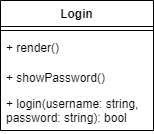
\includegraphics[width=3cm]{img/Architecture/UI/loginUI.png}
    \end{center}
    \caption{Lược đồ class của LoginUI}
\end{figure}
 
Phương thức:
\begin{itemize}
    \item showPassword(): Hiện mật khẩu
    \item login(username: string, password: string)(): Đăng nhập vào hệ thống
\end{itemize}
 
\subsubsection{AdminUI}
Module này bao gồm các class dùng để hiển thị UI đối với phía quản trị viên
 
\begin{figure}[!htp]
    \centering
    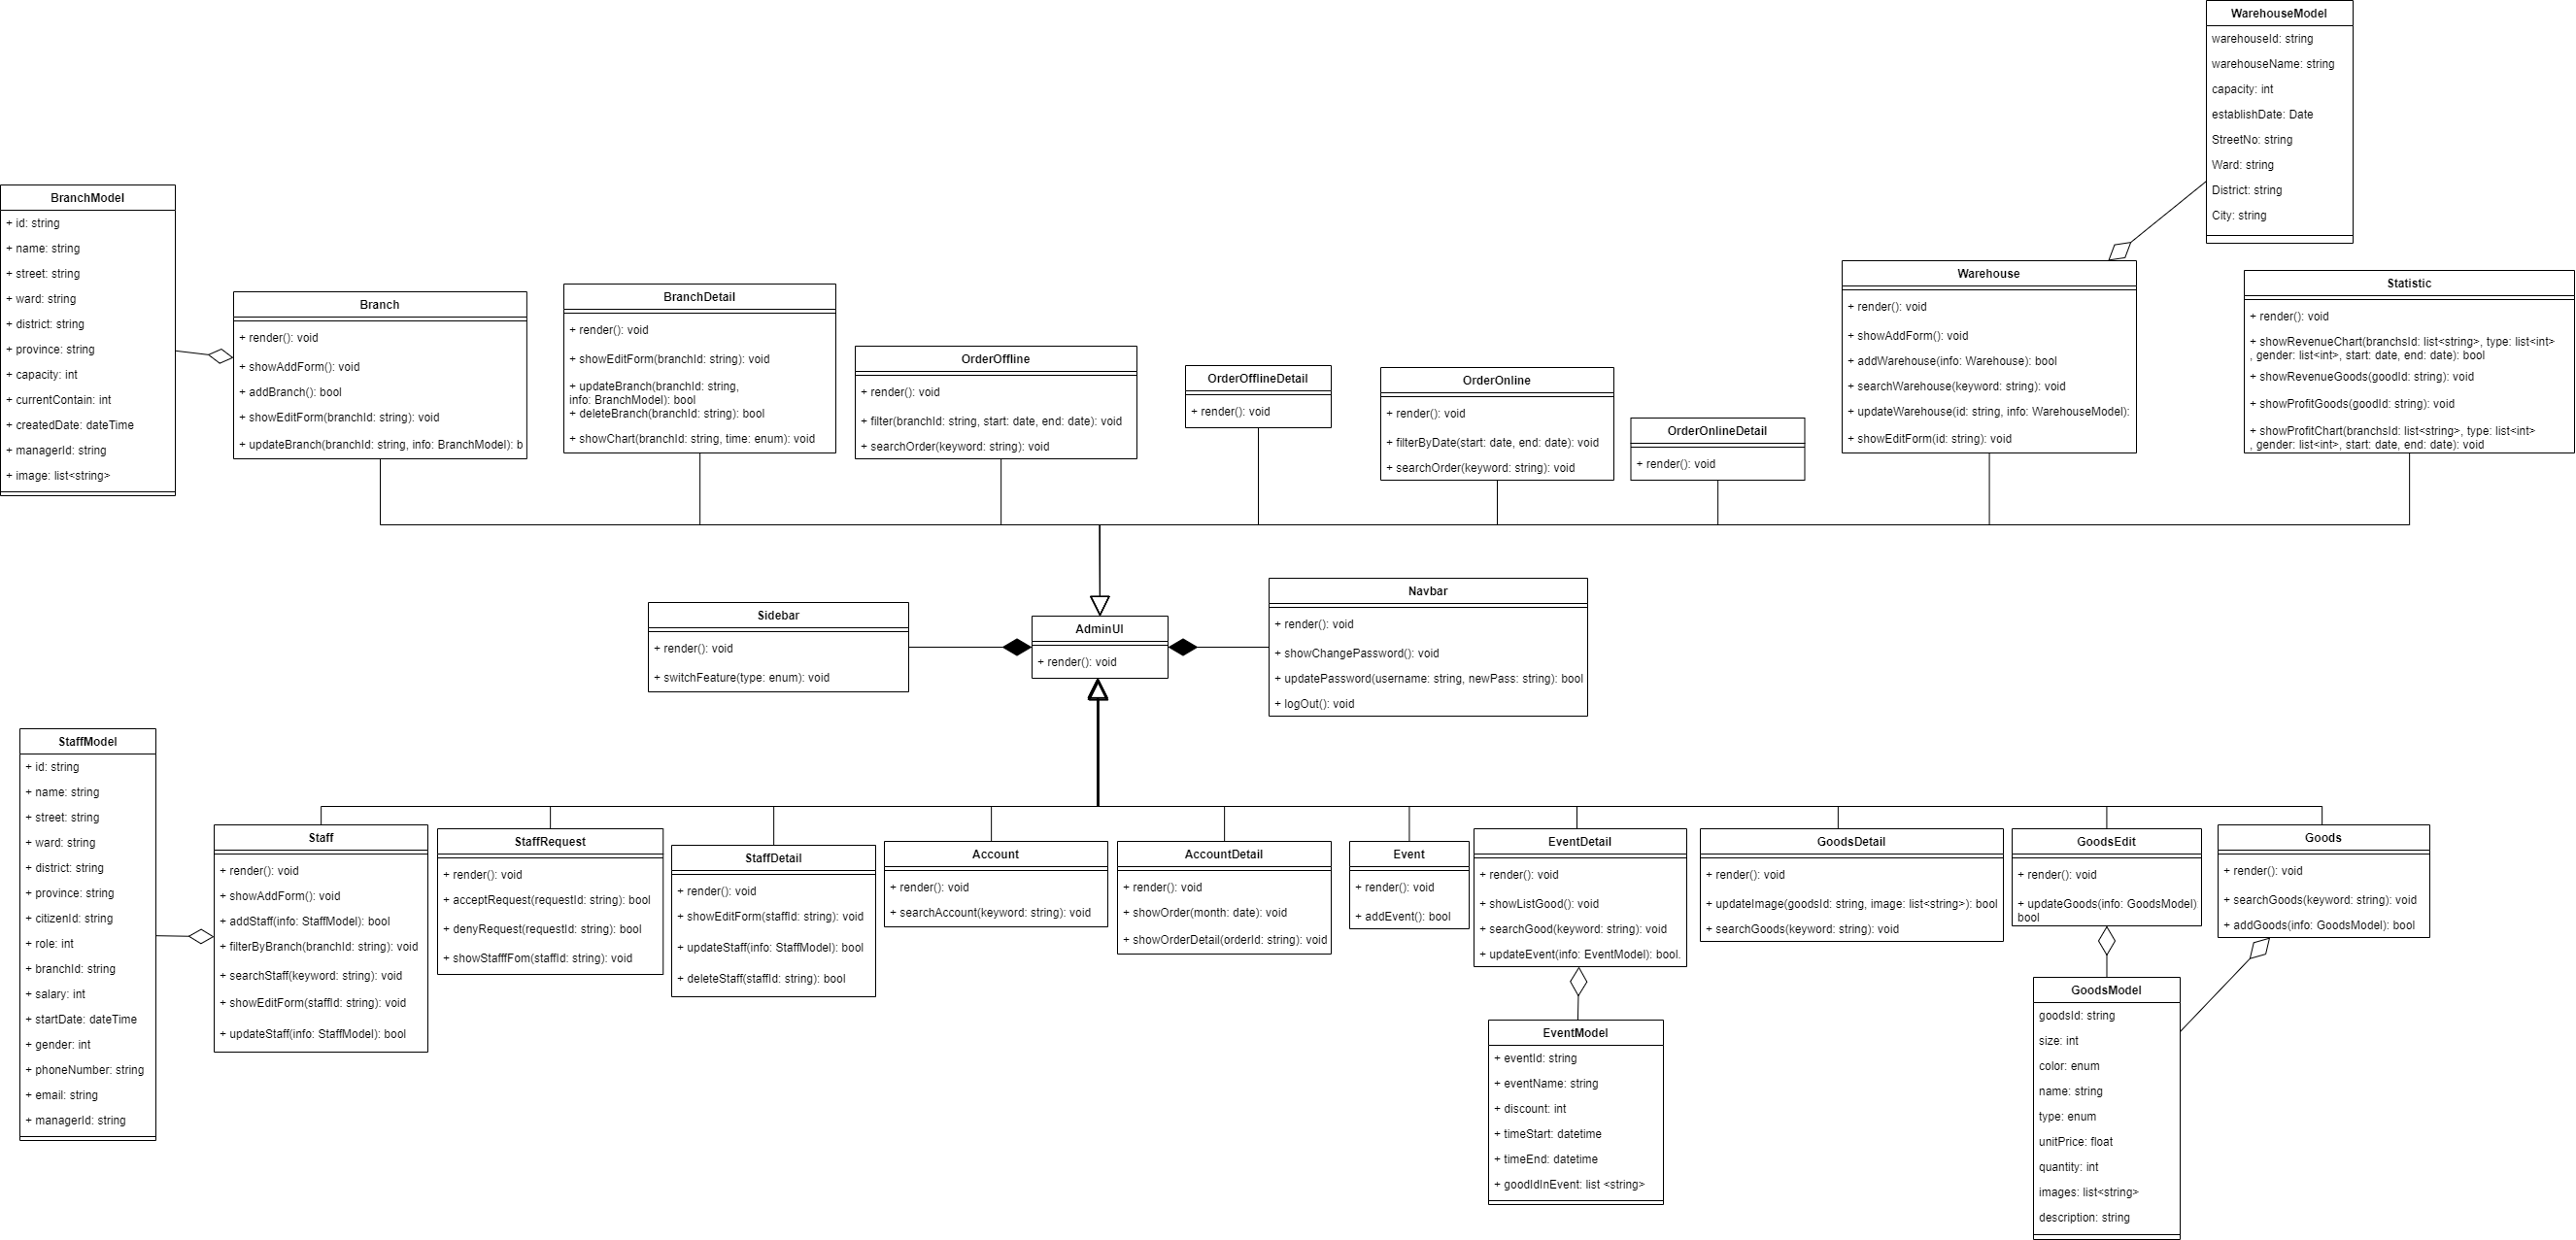
\includegraphics[width=17cm]{img/Architecture/UI/adminUI.png}
    \newline
    \caption{Lược đồ class của Module AdminUI}
\end{figure}
 
\subsubsubsection*{AdminUI}
Phương thức:
\begin{itemize}
    \item render(): Hiển thị màn hình admin
\end{itemize}
 
\subsubsubsection*{Branch}
Màn hình quản lý chi nhánh\\
Phương thức:
\begin{itemize}
    \item showAddForm(): Hiển thị biểu mẫu thêm mới
    \item addBranch(): Thêm chi nhánh mới
    \item showEditForm(branchId: string): Hiển thị biểu mẫu chỉnh sửa
    \item updateBranch(branchId: string, info: BranchModel): Cập nhật thông tin chi nhánh
\end{itemize}
 
\subsubsubsection*{BranchDetail}
Màn hình hiển thị thông tin chi tiết chi nhánh\\
Phương thức:
\begin{itemize}
    \item showEditForm(branchId: string): Hiển thị biểu mẫu chỉnh sửa
    \item updateBranch(branchId: string, info: BranchModel): Cập nhật thông tin chi nhánh
    \item deleteBranch(branchId: string): Xóa chi nhánh
    \item showChart(branchId: string, time: enum): Hiển thị biểu đồ kinh doanh
\end{itemize}
 
\subsubsubsection*{Staff}
Màn hình quản lý nhân viên\\
Phương thức:
\begin{itemize}
    \item showAddForm(): Hiển thị biểu mẫu thêm mới
    \item addStaff(info: StaffModel): Thêm một nhân viên
    \item filterByBranch(branchId: string): Tìm nhân viên theo chi nhánh
    \item searchStaff(keyword: string): Tìm kiếm chi nhánh theo từ khóa
    \item showEditForm(staffId: string): Hiển thị biểu mẫu chỉnh sửa
    \item updateStaff(branchId: string, info: BranchModel): Cập nhật thông tin chi nhánh
\end{itemize}
 
\subsubsubsection*{StaffRequest}
Màn hình quản lý yêu cầu thêm, xóa nhân viên\\
Phương thức:
\begin{itemize}
    \item acceptRequest(requestId: string): Xác nhận yêu cầu
    \item denyRequest(requestId: string): Hủy bỏ yêu cầu
    \item showStafffFom(staffId: string): Hiển thị biểu mẫu thông tin nhân viên
\end{itemize}
 
 
\subsubsubsection*{StaffDetail}
Màn hình hiển thị thông tin chi tiết nhân viên\\
Phương thức:
\begin{itemize}
    \item showEditForm(staffId: string): Hiển thị biểu mẫu chỉnh sửa
    \item updateStaff(info: StaffModel): Cập nhật thông tin nhân viên
    \item deleteBranch(staffId: string): Xóa nhân viên
\end{itemize}
 
\subsubsubsection*{Account}
Màn hình quản lý tài khoản\\
Phương thức:
\begin{itemize}
    \item searchAccount(keyword: string): Tìm kiếm tài khoản theo từ khóa
\end{itemize}
 
 
\subsubsubsection*{AccountDetail}
Màn hình hiển thị thông tin chi tiết tài khoản\\
Phương thức:
\begin{itemize}
    \item showOrder(month: date): Hiển thị danh sách đơn hàng
    \item showOrderDetail(orderId: string): Hiển thị biểu mẫu chi tiết đơn hàng
\end{itemize}
 
\subsubsubsection*{Event}
Màn hình quản lý sự kiện\\
Phương thức:
\begin{itemize}
    \item addEvent(): Thêm một sự kiện mới
\end{itemize}
 
\subsubsubsection*{EventDetail}
Màn hình hiển thị thông tin chi tiết sự kiện\\
Phương thức:
\begin{itemize}
    \item showListGood(): Hiển thị danh sách tất cả hàng
    \item searchGood(keyword: string): Tùm kiếm danh sách hàng theo từ khóa
    \item updateEvent(info: EventModel): Cập nhật thông tin sự kiện
\end{itemize}
 
\subsubsubsection*{Goods}
Màn hình quản lý hàng hóa\\
Phương thức:
\begin{itemize}
    \item searchGoods(keyword: string): Tìm kiếm hàng theo từ khóa
    \item addGoods(info: GoodsModel): Thêm một sản phẩm
\end{itemize}
 
\subsubsubsection*{GoodsDetail}
Màn hình hiển thị thông tin chi tiết hàng hóa\\
Phương thức:
\begin{itemize}
    \item updateImage(goodsId: string, image: list<string>): Cập nhật hình ảnh sản phẩm
    \item searchGoods(keyword: string): Tìm kiếm hàng theo từ khóa
\end{itemize}
 
\subsubsubsection*{GoodsEdit}
Màn hình hiển thị biểu mẫu vận chuyển hàng hóa\\
Phương thức:
\begin{itemize}
    \item updateGoods(info: GoodsModel): Cập nhật thông tin sản phẩm
\end{itemize}
 
\subsubsubsection*{OrderOffline}
Màn hình quản lý các đơn hàng trực tiếp\\
Phương thức:
\begin{itemize}
    \item filter(branchId: string, start: date, end: date): Tìm kiếm đơn hàng theo thời gian, chi nhánh
    \item searchOrder(keyword: string): Tìm kiếm đơn hàng theo từ khóa
\end{itemize}
 
\subsubsubsection*{OrderOnline}
Màn hình quản lý các đơn hàng trực tuyến\\
Phương thức:
\begin{itemize}
    \item filter(start: date, end: date): Tìm kiếm đơn hàng theo thời gian
    \item searchOrder(keyword: string): Tìm kiếm đơn hàng theo từ khóa
\end{itemize}



\subsection{Tầng API}
\subsubsection{Customer APIs}
Module này dùng để chứa các API được xuất ra ngoài cho phía khách hàng:

\subsubsubsection*{Customer Service}
\begin{itemize}
	\item getCustomerInfo
	      \begin{quote}
		      GET: /api/customer-service/customer/{customerId}
		      \begin{itemize}
			      \item customerId: string (Required)
		      \end{itemize}
	      \end{quote}

	\item updateCustomerInfo
	      \begin{quote}
		      PUT /api/customer-service/customer/{customerId}
		      \begin{itemize}
			      \item customerId: string (Required)
			      \item userName: string
			      \item name: string
			      \item phone: string
			      \item gender: string
			      \item ages: string
			      \item street: string
			      \item ward: string
			      \item district: string
			      \item province: string
		      \end{itemize}
	      \end{quote}

	\item addCustomerInfo
	      \begin{quote}
		      POST /api/customer-service/customer
		      \begin{itemize}
			      \item userName: string (Required)
			      \item name: string (Required)
			      \item phone: string (Required)
			      \item password: string (Required)
		      \end{itemize}
	      \end{quote}
\end{itemize}

\subsubsubsection*{Cart Service}
\begin{itemize}
	\item addCart
	      \begin{quote}
		      POST /api/cart-service/cart
		      \begin{itemize}
			      \item customerId: string (Required)
		      \end{itemize}
	      \end{quote}

	\item getCart
	      \begin{quote}
		      GET /api/cart-service/cart/{customerId}
		      \begin{itemize}
			      \item customerId: string (Required)
		      \end{itemize}
	      \end{quote}

	\item addProductToCart
	      \begin{quote}
		      POST /api/cart-service/cart/{customerId}
		      \begin{itemize}
			      \item cartId: string (Required)
			      \item product: GoodsInCart (Required)\\
							GoodInCart:
							\begin{itemize}
								\item goodsId: string 
								\item color: string 
								\item size: string 
								\item quantity: string 
							\end{itemize}
		      \end{itemize}
	      \end{quote}

	\item removeProductToCart
	      \begin{quote}
		      DELETE /api/cart-service/cart/{cartId}
		      \begin{itemize}
			      \item cartId: string (Required)
			      \item product: Goods (Required)\\
							Goods:
							\begin{itemize}
								\item goodsId: string 
								\item color: string 
								\item size: string
							\end{itemize}
		      \end{itemize}
	      \end{quote}

	\item removeAllProductInCart
	      \begin{quote}
		      DELETE /api/cart-service/cart/all/{cartId}
		      \begin{itemize}
			      \item cartId: string (Required)
		      \end{itemize}
	      \end{quote}

	\item UpdateCart
	      \begin{quote}
		      PUT /api/cart-service/cart/{cartId}
		      \begin{itemize}
			      \item cartId: string (Required)
			      \item product: GoodsInCart (Required)\\
							GoodInCart:
							\begin{itemize}
								\item goodsId: string 
								\item color: string 
								\item size: string 
								\item quantity: string 
							\end{itemize}
		      \end{itemize}
	      \end{quote}
\end{itemize}

\subsubsubsection*{Customer Order Service}
\begin{itemize}
	\item getListOrder
	      \begin{quote}
		      GET /api/order-service/orders/{customerId}
		      \begin{itemize}
			      \item customerId: string (Required)
		      \end{itemize}
	      \end{quote}

	\item getOrderDetail
	      \begin{quote}
		      GET /api/order-service/order-detail
		      \begin{itemize}
			      \item customerId: string (Required)
			      \item orderId: string (Required)
		      \end{itemize}
	      \end{quote}

	\item makeOrder
	      \begin{quote}
		      POST /api/make-order-service/order
		      \begin{itemize}
			      \item transactionDate: DateTime (Required)
			      \item totalAmount: float (Required)
			      \item isOnline: bool (Required)
			      \item customerId: string (Required when isOnline == true)
			      \item shippingFee: float (Required when isOnline == true)
			      \item storeId: string (Required when isOnline == false)
			      \item goods: [GoodsInOrder] (Required)\\
							GoodsInOrder:
							\begin{itemize}
								\item goodsId: string 
								\item color: string 
								\item size: string 
								\item quantity: string 
								\item unitPrice: float 
								\item taxAmount: float 
								\item totalPrice: float 
								\item description: string
							\end{itemize}
		      \end{itemize}
	      \end{quote}
	\item calcShipFee
	      \begin{quote}
		      POST /api/make-order-service/ship-fee
		      \begin{itemize}
			      \item address: Address (Required)\\
							Address:
							\begin{itemize}
								\item street: string 
								\item ward: string
								\item district: string
								\item province: string
							\end{itemize}
		      \end{itemize}
	      \end{quote}
	\item makePayment
	      \begin{quote}
		      POST /api/make-order-service/payment
		      \begin{itemize}
			      \item cost: float (Required)
		      \end{itemize}
	      \end{quote}			
\end{itemize}

\subsubsubsection*{Order Service}
\begin{itemize}
	\item readOrder
	      \begin{quote}
		      GET /api/order-service/order/{orderId}
		      \begin{itemize}
			      \item orderId: string (Required)
		      \end{itemize}
	      \end{quote}

	\item createOrder
	      \begin{quote}
		      POST /api/order-service/order
		      \begin{itemize}
			      \item transactionDate: DateTime (Required)
			      \item totalAmount: int (Required)
			      \item isOnline: bool (Required)
			      \item customerId: string
			      \item shippingFee: float
			      \item storeId: string
			      \item goods: [GoodsInOrder] (Required)
		      \end{itemize}
	      \end{quote}

	\item readOnlineOrderStatus
	      \begin{quote}
		      GET /api/order-service/online-order-status/{orderId}
		      \begin{itemize}
			      \item orderId: string (Required)
		      \end{itemize}
	      \end{quote}

	\item getOrderDetail
	      \begin{quote}
		      GET /api/order-service/order-detail
		      \begin{itemize}
			      \item customerId: string (Required)
			      \item orderId: string (Required)
		      \end{itemize}
	      \end{quote}
\end{itemize}

\subsubsubsection*{Account Service}
\begin{itemize}
	\item Authentication
	      \begin{quote}
		      GET /api/account-service/{username}
		      \begin{itemize}
			      \item password: string (Required)
		      \end{itemize}
	      \end{quote}

	\item addAccount
	      \begin{quote}
		      POST /api/account-service/add
		      \begin{itemize}
			      \item password: string (Required)
			      \item username: string (Required)
			      \item role: enum (Required)
		      \end{itemize}
	      \end{quote}
\end{itemize}





\subsubsection{Admin APIs}
Module này dùng để chứa các API được xuất ra ngoài cho phía quản trị viên

\subsubsubsection*{Event Service}
\begin{itemize}
	\item addEvent
	      \begin{quote}
		      POST /api/event-service/event
		      \begin{itemize}
			      \item event: EventModel (Required)
		      \end{itemize}
	      \end{quote}

	\item getAllEvent
	      \begin{quote}
		      GET /api/event-service/event
	      \end{quote}

	\item removeEvent
	      \begin{quote}
		      DELETE /api/event-service/event/{eventId}
		      \begin{itemize}
			      \item eventId: string (Required)
		      \end{itemize}
	      \end{quote}

	\item UpdateEvent
	      \begin{quote}
		      PUT /api/event-service/event/{eventId}
		      \begin{itemize}
			      \item eventId: string (Required)
			      \item event: EventModel (Required)
		      \end{itemize}
	      \end{quote}
\end{itemize}

\subsubsubsection*{Warehouse Service}
\begin{itemize}
	\item getManager
	      \begin{quote}
		      GET /api/warehouse-service/manager/{warehouseId}
	      \end{quote}

	\item updateManager
	      \begin{quote}
		      PUT /api/warehouse-service/manager
			  \begin{itemize}
				\item managerId: string (Required)
				\item warehouseId: string (Required)
			\end{itemize}
	      \end{quote}

	\item getStaff
	      \begin{quote}
		      GET /api/warehouse-service/staff/{warehouseId}
	      \end{quote}

	\item addStaff
	      \begin{quote}
		      POST /api/warehouse-service/staff
			  \begin{itemize}
				\item staffId: string (Required)
				\item warehouseId: string (Required)
			\end{itemize}
	      \end{quote}

	\item updateStaff
	      \begin{quote}
		      PUT /api/warehouse-service/staff
			  \begin{itemize}
				\item managerId: string (Required)
				\item warehouseId: string (Required)
			\end{itemize}
	      \end{quote}

	\item deleteStaff
	      \begin{quote}
		      DELETE /api/warehouse-service/staff
			  \begin{itemize}
				\item managerId: string (Required)
			\end{itemize}
	      \end{quote}

	\item addWarehouse
	      \begin{quote}
		      POST /api/warehouse-service/warehouse
			  \begin{itemize}
				\item warehouseId: string (Required)
				\item warehouseName: string (Required)
				\item capacity: int (Required)
				\item established\_date: Date
				\item street\_no: string (Required)
				\item ward: string (Required)
				\item district: string (Required)
				\item city: string (Required)
			\end{itemize}
	      \end{quote}

	\item getWarehouse
	      \begin{quote}
		      GET /api/warehouse-service/warehouse/{warehouseId}
	      \end{quote}

	\item updateWarehouse
	      \begin{quote}
		      PUT /api/warehouse-service/warehouse
			  \begin{itemize}
				\item warehouseId: string (Required)
				\item warehouseName: string (Required)
				\item capacity: int (Required)
				\item established\_date: Date
				\item street\_no: string (Required)
				\item ward: string (Required)
				\item district: string (Required)
				\item city: string (Required)
			\end{itemize}
	      \end{quote}

	\item deleteWarehouse
	      \begin{quote}
		      DELETE /api/warehouse-service/warehouse
			  \begin{itemize}
				\item warehouseId: string (Required)
			\end{itemize}
	      \end{quote}
\end{itemize}

\subsubsubsection*{Goods Service}
\begin{itemize}
	\item getGoods
	      \begin{quote}
		      GET /api/goods-service/goods{goodsId}
		      \begin{itemize}
			      \item goods\_code: string (Required)
		      \end{itemize}
	      \end{quote}

	\item updateGoods
	      \begin{quote}
		      PUT /api/goods-service/goods
			  \begin{itemize}
				\item goods\_code: string (Required)
				\item size: string (Required)
				\item color: string (Required)
				\item goods\_name: string (Required)
				\item type: string (Required)
				\item gender: int (Required)
				\item age: string (Required)
				\item manufacturer: string (Required)
				\item for\_sale: bool
				\item unit\_price: int (Required)
				\item description: string
			  \end{itemize}
	      \end{quote}

	\item addGoods
	      \begin{quote}
		      POST /api/goods-service/goods
			  \begin{itemize}
				\item goods\_code: string (Required)
				\item size: string (Required)
				\item color: string (Required)
				\item goods\_name: string (Required)
				\item type: string (Required)
				\item gender: int (Required)
				\item age: string (Required)
				\item manufacturer: string (Required)
				\item for\_sale: bool
				\item unit\_price: int (Required)
				\item description: string
			  \end{itemize}
	      \end{quote}

	\item deleteGoods
	      \begin{quote}
		      DELETE /api/goods-service/goods
			  \begin{itemize}
				\item goods\_code: string (Required)
			  \end{itemize}
	      \end{quote}

	\item createImport
	      \begin{quote}
		      POST /api/goods-service/import
			  \begin{itemize}
				\item goods\_code: string (Required)
				\item dest\_warehouse: string (Required)
				\item quantity: int (Required)
			  \end{itemize}
	      \end{quote}

	\item createExport
	      \begin{quote}
		      POST /api/goods-service/export
			  \begin{itemize}
				\item goods\_code: string (Required)
				\item source\_warehouse: string (Required)
				\item quantity: int (Required)
			  \end{itemize}
	      \end{quote}

	\item createWHTransfer
	      \begin{quote}
		      POST /api/goods-service/wh-transfer
			  \begin{itemize}
				\item goods\_code: string (Required)
				\item source\_warehouse: string (Required)
				\item dest\_warehouse: string (Required)
				\item quantity: int (Required)
			  \end{itemize}
	      \end{quote}

	\item createReturnManufact
	      \begin{quote}
		      POST /api/goods-service/return-manufact
			  \begin{itemize}
				\item goods\_code: string (Required)
				\item source\_warehouse: string (Required)
				\item manufacturer: string (Required)
				\item quantity: int (Required)
			  \end{itemize}
	      \end{quote}

	\item createCustReturn
	      \begin{quote}
		      POST /api/goods-service/cust-return
			  \begin{itemize}
				\item goods\_code: string (Required)
				\item dest\_warehouse: string (Required)
				\item quantity: int (Required)
			  \end{itemize}
	      \end{quote}
\end{itemize}

\subsubsubsection*{Branch Service}
\begin{itemize}
	\item readListBranch
	\begin{quote}
		GET /api/branch-service/
	\end{quote}


	\item readBranchDetail
	\begin{quote}
		GET /api/branch-service/{branchId}
	\end{quote}

	\item updateBranch
	\begin{quote}
		PUT /api/branch-service/statistic/{branchId}
		\begin{itemize}
			\item name: string
			\item capacity: int 
			\item address: string
			\item open: dateTime
			\item close: dateTime
		\end{itemize}
	\end{quote}

	\item updateBranchManager
	\begin{quote}
		PUT /api/branch-service/manager/{branchId}
		\begin{itemize}
			\item staffId: string (Required)
		\end{itemize}
	\end{quote}

	\item addBranch
	\begin{quote}
		POST /api/branch-service/
		\begin{itemize}
			\item name: string (Required)
			\item capacity: int (Required)
			\item address: string (Required)
			\item open: dateTime (Required)
			\item close: dateTime (Required)
		\end{itemize}
	\end{quote}

	\item deleteBranch
	\begin{quote}
		DELETE /api/branch-service/{branchId}
	\end{quote}

	\item readBranchStaff
	\begin{quote}
		GET /api/branch-service/staff/{branchId}
	\end{quote}

	\item readBranchStatistic
	\begin{quote}
		GET /api/branch-service/statistic/{branchId}
		\begin{itemize}
			\item time: enum (Required)
		\end{itemize}
	\end{quote}
\end{itemize}

\subsubsubsection*{Account Service}
\begin{itemize}
	\item readListAccount
	\begin{quote}
		GET /api/account-service/
	\end{quote}

	\item Authentication
	\begin{quote}
		GET /api/account-service/{username}
		\begin{itemize}
			\item password: string (Required)
		\end{itemize}
	\end{quote}

	\item filterAccount
	\begin{quote}
		GET /api/account-service?keyword=\{keyword\}
	\end{quote}

	\item updateRole
	\begin{quote}
		PUT /api/account-service/role/{username}
		\begin{itemize}
			\item role: enum (Required)
		\end{itemize}
	\end{quote}

	\item addAccount
	\begin{quote}
		POST /api/account-service/add
		\begin{itemize}
			\item password: string (Required)
			\item username: string (Required)
			\item role: enum (Required)
		\end{itemize}
	\end{quote}
\end{itemize}

\subsubsubsection*{Staff Service}
\begin{itemize}
	\item readListStaff
	\begin{quote}
		GET /api/staff-service/staff
	\end{quote}

	\item readDetailStaff
	\begin{quote}
		GET /api/staff-service/staff/{staffId}
	\end{quote}

	\item getAttendanceStaff
	\begin{quote}
		GET /api/staff-service/staff/attendance/{staffId}
	\end{quote}

	\item filterStaff
	\begin{quote}
		GET /api/staff-service/staff?keyword=\{keyword\}
	\end{quote}

	\item addStaff
	\begin{quote}
		POST /api/staff-service/staff
		\begin{itemize}
			\item name: string (Required)
			\item birthDate: date (Required)
			\item homeTown: string (Required)
			\item citizenId: string (Required)
			\item phone: string (Required)
			\item address: string (Required)
			\item workingPlace: enum (Required)
			\item role: enum (Required)
			\item salary: int (Required)
			\item username: enum
			\item password: enum
		\end{itemize}
	\end{quote}

	\item updateStaff
	\begin{quote}
		PUT /api/staff-service/staff/{staffId}
		\begin{itemize}
			\item birthDate: date
			\item homeTown: string
			\item citizenId: string
			\item phone: string
			\item address: string
			\item workingPlace: enum
			\item role: enum
			\item salary: int
			\item username: enum
			\item password: enum
		\end{itemize}
	\end{quote}

	\item deleteStaff
	\begin{quote}
		DELETE /api/staff-service/staff/{staffId}
	\end{quote}

	\item createAddRequest
	\begin{quote}
		POST /api/staff-service/request/add
		\begin{itemize}
			\item name: string (Required)
			\item birthDate: date (Required)
			\item homeTown: string (Required)
			\item citizenId: string (Required)
			\item phone: string (Required)
			\item address: string (Required)
			\item workingPlace: enum (Required)
			\item role: enum (Required)
			\item salary: int (Required)
		\end{itemize}
	\end{quote}

	\item createDeleteRequest
	\begin{quote}
		POST /api/staff-service/request/delete/{staffId}
	\end{quote}

	\item updateRequestStatus
	\begin{quote}
		PUT /api/staff-service/request/{requestId}
		\begin{itemize}
			\item status: bool (Required)
		\end{itemize}
	\end{quote}

\end{itemize}

\subsubsubsection*{Statistic Service}
\begin{itemize}
	\item getStatistic
	\begin{quote}
		GET /api/statistic-service
		\begin{itemize}
			\item start: dateTime (Required)
			\item end: dateTime (Required)
		\end{itemize}
	\end{quote}

	\item getRevenue
	\begin{quote}
		GET /api/statistic-service/revenue
		\begin{itemize}
			\item branchId: string
			\item gender: enum
			\item type: enum
			\item start: dateTime (Required)	
			\item end: dateTime (Required)
		\end{itemize}
	\end{quote}

	\item getRevenue1Goods
	\begin{quote}
		GET /api/statistic-service/revenue/{goodsId}
		\begin{itemize}
			\item start: dateTime (Required)	
			\item end: dateTime (Required)
		\end{itemize}
	\end{quote}

	\item getProfit
	\begin{quote}
		GET /api/statistic-service/profit
		\begin{itemize}
			\item branchId: string
			\item gender: enum
			\item type: enum
			\item start: dateTime (Required)	
			\item end: dateTime (Required)
		\end{itemize}
	\end{quote}

	\item getProfit1Goods
	\begin{quote}
		GET /api/statistic-service/profit/{goodsId}
		\begin{itemize}
			\item start: dateTime (Required)	
			\item end: dateTime (Required)
		\end{itemize}
	\end{quote}

\end{itemize}



\subsubsection{Shared APIs}
Module này dùng để chứa các API được xuất ra ngoài cho bất kì đối tượng người dùng nào

\subsubsubsection*{Goods Service}
\begin{itemize}
	\item getGoods
	      \begin{quote}
		      GET /api/goods-service/goods{goodsId}
		      \begin{itemize}
			      \item goodsId: string (Required)
		      \end{itemize}
	      \end{quote}
\end{itemize}



\subsection{Tầng Web Service}
 
Lược đồ class ở tầng Web Service được xây dựng theo các thành phần sau:
\begin{itemize}
    \item Repository: Class dùng để truy cập trực tiếp đến dữ liệu trong Database
    \item Model: Class dùng để chứa thông tin nhận lên từ Database
    \item Controllers: Class dùng để xử lý các logic nghiệp vụ
    \item Response: Class chứa thông tin trả về khi có yêu cầu từ bên ngoài
    \item Các Interface: Giúp đảm bảo nguyên lý \textbf{Dependency inversion principle} của \textbf{SOLID}
    \begin {itemize}
        \item IRepository: Cung cấp các api cho các class Controller
        \item IController: Cung cấp các api để bên ngoài dịch vụ web truy cập đến
    \end{itemize}
\end{itemize}

\newpage

\subsubsection{Customer Order Service}
\begin{figure}[!htp]
	\centering
	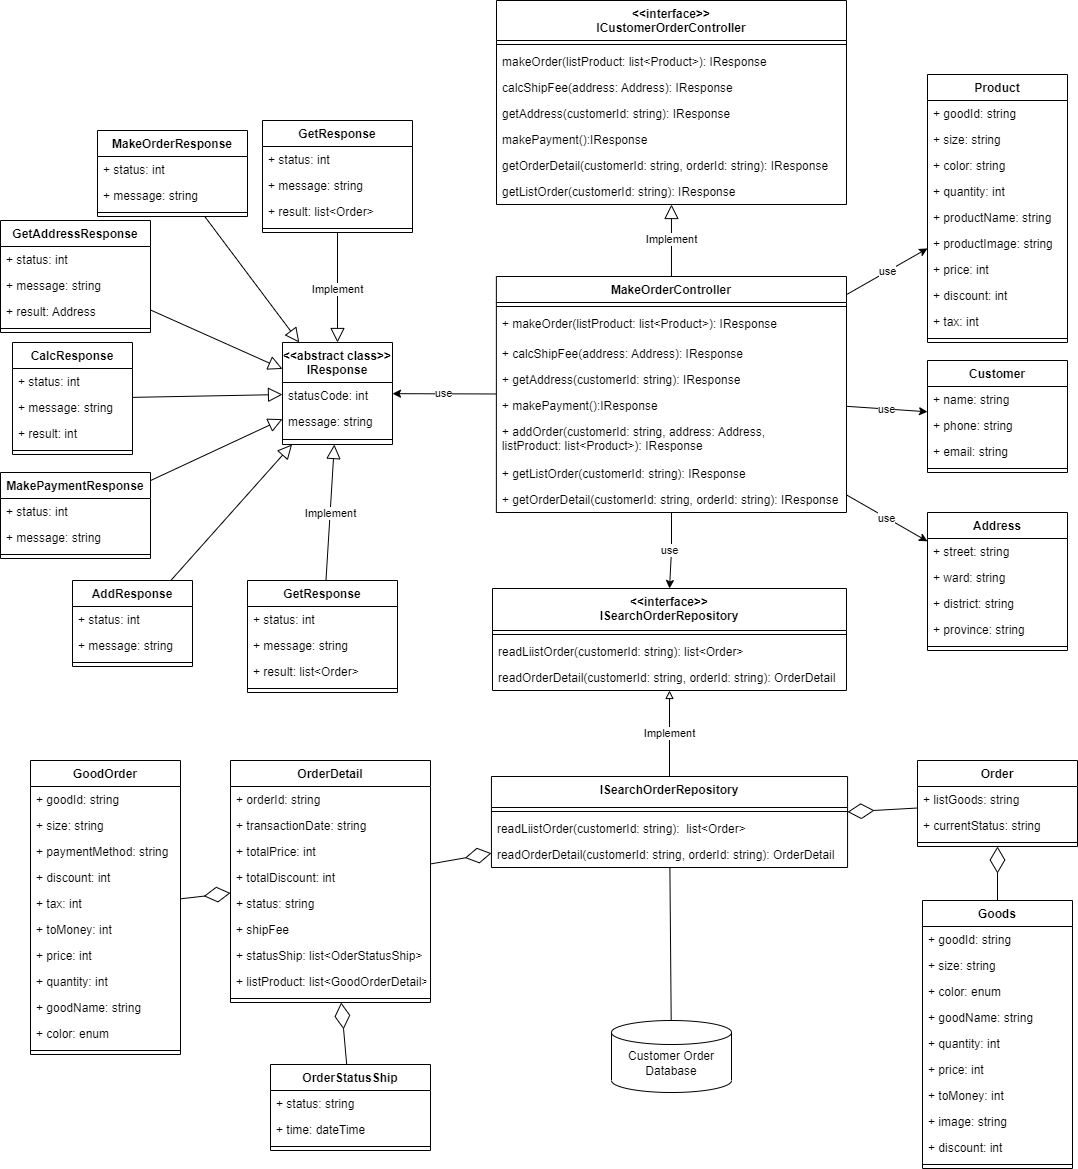
\includegraphics[width=13cm]{img/Architecture/service/CustomerOrderService.png}
	\newline
	\caption{Lược đồ class của Customer Order Service}
\end{figure}

\subsubsubsection*{CustomerOrderRepository}
Thuộc tính:
\begin{itemize}
	\item order: Chứa đối tượng Order
	\item orderDetail: Chứa đối tượng OrderDetail
\end{itemize}
Phương thức:
\begin{itemize}
	\item readListOrder(customerId: string): Lấy danh sách đơn hàng theo mã khách hàng
	\item readOrderDetail(customerId: string, orderId: string): Lấy thông tin chi tiết của đơn hàng.
\end{itemize}

\subsubsubsection*{CustomerOrderController}
Thuộc tính:
\begin{itemize}
	\item repo: Chứa đối tượng CustomerOrderRepository
\end{itemize}
Phương thức:
\begin{itemize}
	\item makeOrder(listProduct: list<Product>): Tạo đơn hàng
	\item calcShipFee(address: Address): Tính chi phí giao hàng
	\item getAddress(customerId: string): Lấy thông tin địa chỉ của tài khoản của khách hàng.
	\item makePayment(customerId: string): Tạo giao dịch thanh toán.
	\item addOrder(customerId: string, address: Address, listProduct: list<Product>): Thêm đơn hàng vào cơ sở dữ liệu của hệ thống.
	\item getListOrder(customerId: string): Lấy danh sách đơn hàng theo mã khách hàng
	\item getOrderDetail(customerId: string, orderId: string): Lấy thông tin chi tiết của đơn hàng.
\end{itemize}

\subsubsubsection*{MakeOrderResponse - GetAddressResponse - CalcResponse - MakePaymentResponse - AddResponse}
Thuộc tính:
\begin{itemize}
	\item statusCode: Mã trạng thái của phản hồi
	\item message: Thông điệp của phản hồi
	\item value: Các dữ liệu trả về đối với các yêu cầu
\end{itemize}

\newpage


\subsubsection{Cart Service}
\begin{figure}[!htp]
	\centering
	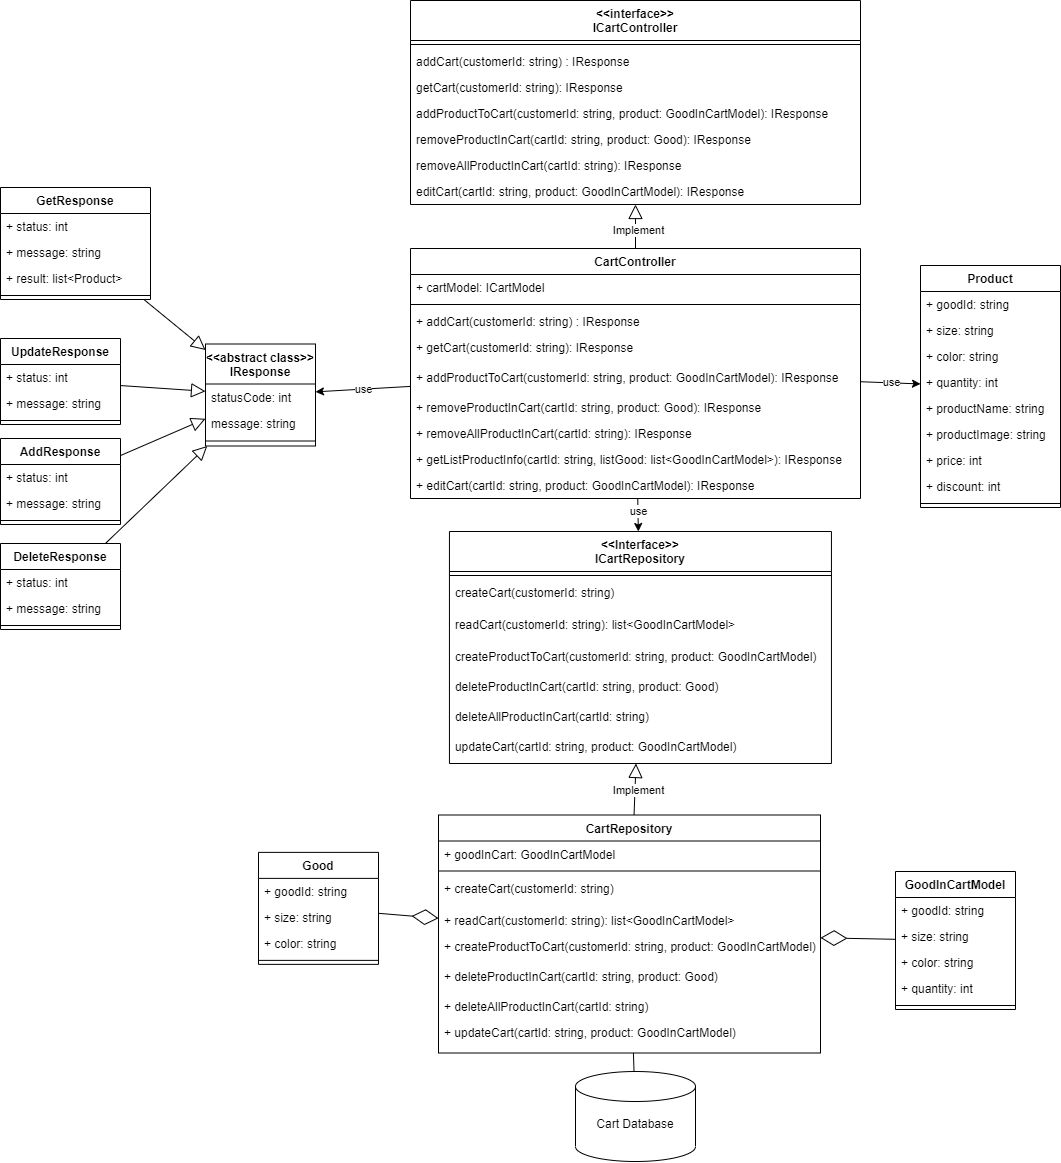
\includegraphics[width=11cm]{img/Architecture/service/CartService.png}
	\newline
	\caption{Lược đồ class của Cart Service}
\end{figure}

\subsubsubsection*{CartRepository}
Thuộc tính:
\begin{itemize}
	\item goodInCart: Chứa đối tượng GoodInCartModel
\end{itemize}
Phương thức:
\begin{itemize}
	\item createCart(customerId: string): tạo giỏ hàng cho tài khoản khách hàng
	\item readCart(customerId: string): Lấy thông tin giỏ hàng thuộc tài khoản của khách hàng.
	\item createProductToCart(customerId: string, product: GoodInCartModel): Thêm sản phẩm vào giỏ hàng.
	\item deleteProductInCart(cartId: string, product: Good): Xóa sản phẩm khỏi giỏ hàng.
	\item deleteAllProductInCart(cartId: string): Xóa toàn bộ sản phẩm khỏi giỏ hàng.
	\item updateCart(customerId: string, product: GoodInCartModel): Cập nhật thông tin sản phẩm trong giỏ hàng.
\end{itemize}

\subsubsubsection*{CartController}
Thuộc tính:
\begin{itemize}
	\item repo: Chứa đối tượng CartRepository
\end{itemize}
Phương thức:
\begin{itemize}
	\item addCart(customerId: string): Xử lý dữ liệu và gọi thêm giỏ hàng cho tài khoản khách hàng để trả về kết quả.
	\item getCart(customerId: string): Xử lý dữ liệu và gọi lấy thông tin giỏ hàng thuộc tài khoản của khách hàng để trả về kết quả.
	\item addProductToCart(customerId: string, product: GoodInCartModel): Xử lý dữ liệu và gọi thêm sản phẩm vào giỏ hàng để trả về kết quả.
	\item removeProductInCart(cartId: string, product: Good): Xử lý dữ liệu và gọi xóa sản phẩm khỏi giỏ hàng để trả về kết quả.
	\item removeAllProductInCart(castId: string): Xử lý dữ liệu và gọi xóa toàn bộ sản phẩm khỏi giỏ hàng để trả về kết quả.
	\item getListProductInfo(cartId: string, listGood: list<GoodInCartModel>): Xử lý dữ liệu và gọi xóa toàn bộ sản phẩm khỏi giỏ hàng để trả về kết quả.
	\item editCart(cartId: string, product: GoodInCartModel): Xử lý dữ liệu và gọi cập nhật thông tin sản phẩm trong giỏ hàng để trả về kết quả.
\end{itemize}

\subsubsubsection*{GetResponse - AddResponse - UpdateResponse - DeleteResponse}
Thuộc tính:
\begin{itemize}
	\item statusCode: Mã trạng thái của phản hồi.
	\item message: Thông điệp của phản hồi.
	\item value: Các dữ liệu trả về đối với các yêu cầu.
\end{itemize}

\newpage


\subsubsection{Customer Service}
\begin{figure}[!htp]
	\centering
	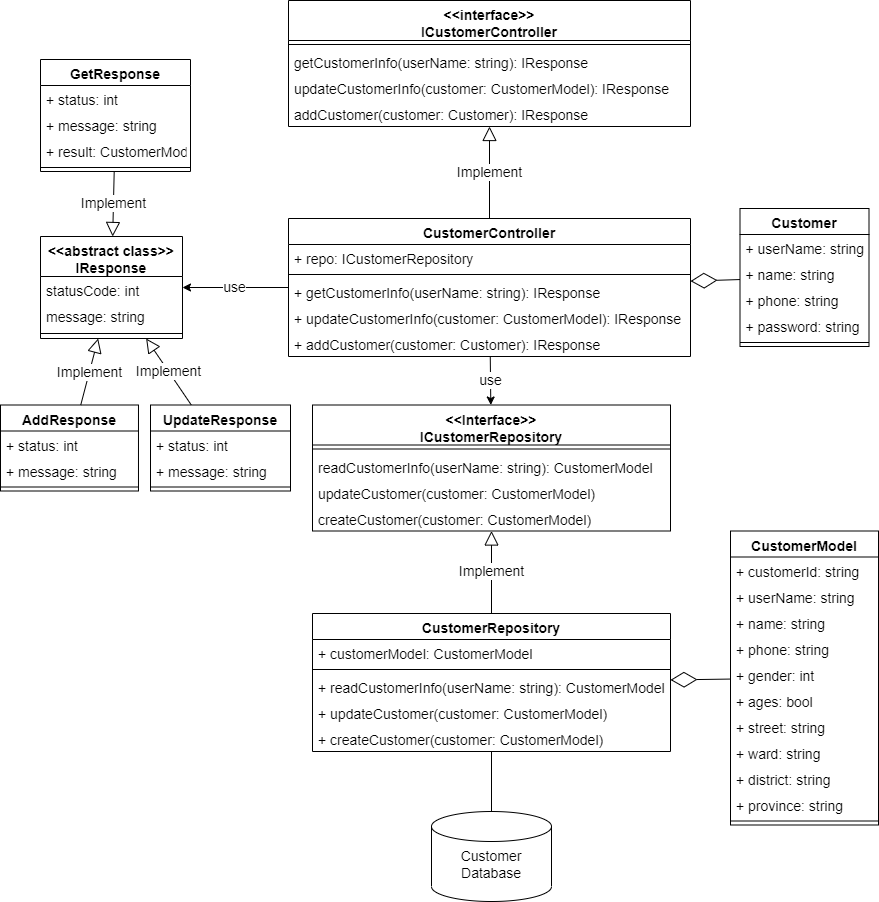
\includegraphics[width=11cm]{img/Architecture/service/CustomerService.png}
	\newline
	\caption{Lược đồ class của Customer Service}
\end{figure}

\subsubsubsection*{CustomerRepository}
Thuộc tính:
\begin{itemize}
	\item customerModel: Chứa đối tượng CustomerModel
\end{itemize}
Phương thức:
\begin{itemize}
	\item createCustomer(customer: CustomerModel): tạo tài khoản khách hàng
	\item updateCustomer(customer: CustomerModel): cập nhật tài khoản khách hàng
	\item readCustomerInfo(username: string): lấy thông tin chi tiết của tài khoản khách hàng
\end{itemize}

\subsubsubsection*{CustomerController}
Thuộc tính:
\begin{itemize}
	\item repo: Chứa đối tượng CustomerRepository
\end{itemize}
Phương thức:
\begin{itemize}
	\item createCustomer(customer: CustomerModel): Xử lý dữ liệu và gọi tạo tài khoản khách hàng để trả về kết quả.
	\item updateCustomer(customer: CustomerModel): Xử lý dữ liệu và gọi cập nhật tài khoản khách hàng để trả về kết quả.
	\item readCustomerInfo(username: string): Xử lý dữ liệu và gọi lấy thông tin chi tiết của tài khoản khách hàng để trả về kết quả.
\end{itemize}

\subsubsubsection*{GetResponse - AddResponse - UpdateResponse}
Thuộc tính:
\begin{itemize}
	\item statusCode: Mã trạng thái của phản hồi
	\item message: Thông điệp của phản hồi
	\item value: Các dữ liệu trả về đối với các yêu cầu
\end{itemize}

\newpage


\subsubsection{Order Service}
\begin{figure}[!htp]
	\centering
	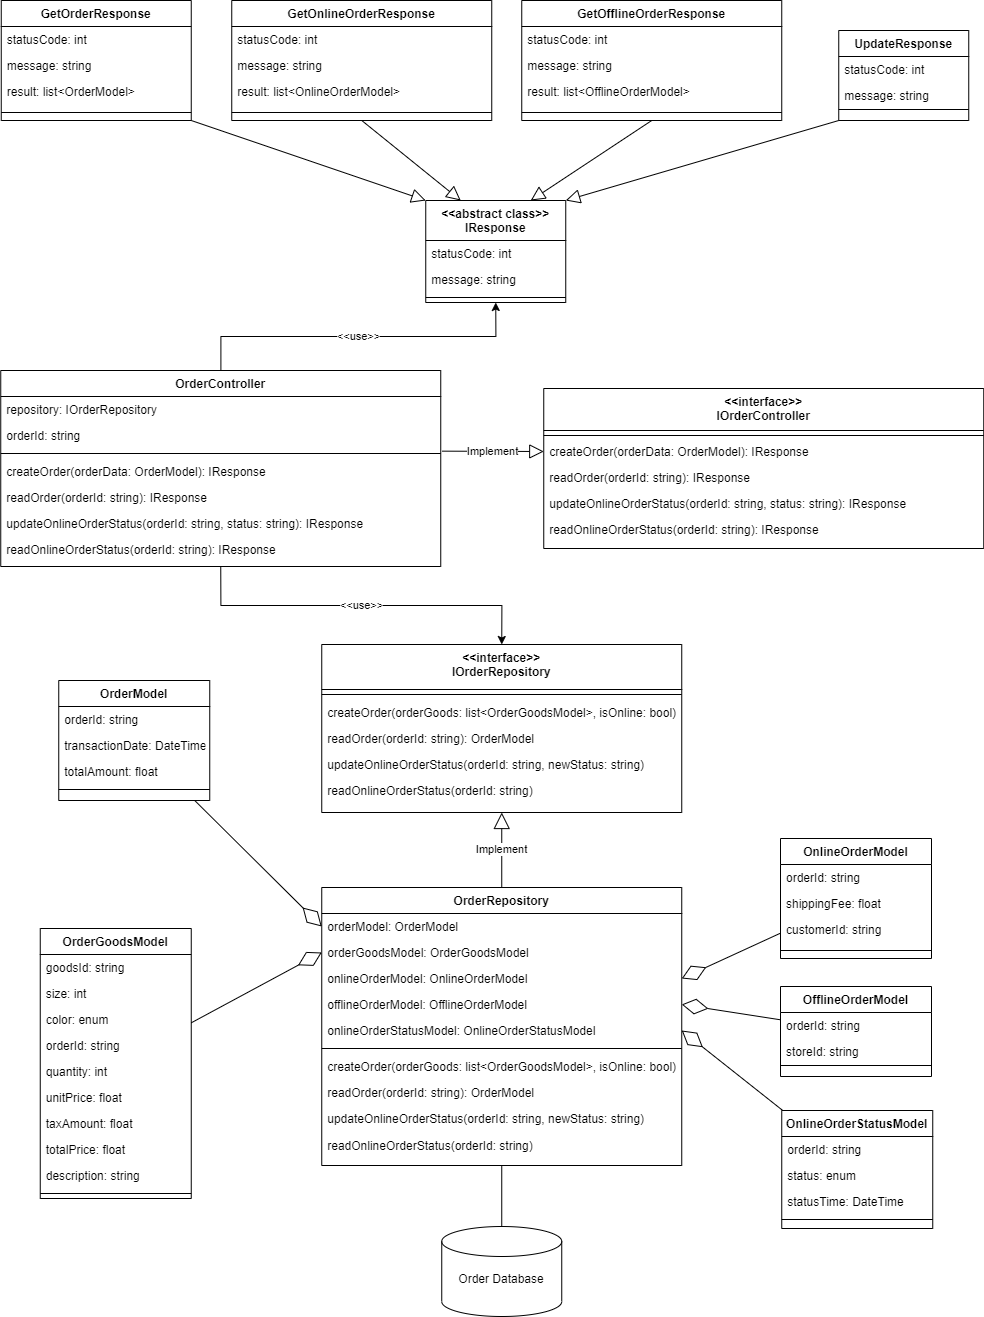
\includegraphics[width=11cm]{img/Architecture/service/OrderService.png}
	\newline
	\caption{Lược đồ class của Order Service}
\end{figure}
\subsubsubsection*{OrderRepository}
Thuộc tính:
\begin{itemize}
	\item orderModel: chứa đối tượng OrderModel
	\item orderGoodsModel: chứa đối tượng OrderGoodsModel
	\item onlineOrderModel: chứa đối tượng OnlineOrderModel
	\item offlineOrderModel: chứa đối tượng OfflineOrderModel 
	\item onlineOrderStatusModel: chứa đối tượng OnlineOrderStatusModel
\end{itemize}
Phương thức:
\begin{itemize}
	\item createOrder(orderGoods: list<OrderGoodsModel>): Tạo đơn hàng.
	\item readOrder(orderId: string): Lấy thông tin đơn hàng.
	\item updateOnlineOrderStatus(orderId: string, status: string): Cập nhật trạng thái đơn hàng.
	\item readOnlineOrderStatus(orderId: string): Lấy thông tin trạng thái đơn hàng.
\end{itemize}

\subsubsubsection*{OrderController}
Thuộc tính:
\begin{itemize}
	\item repository: Chứa đối tượng IOrderRepository
	\item orderId: mã đơn hàng
\end{itemize}
Phương thức:
\begin{itemize}
	\item createOrder(orderData: OrderModel): tạo đơn hàng.
	\item readOrder(orderId: string): Lấy dữ liệu đơn hàng.
	\item updateOnlineOrderStatus(orderId: string, status: string): Cập nhật trạng thái đơn hàng.
	\item readOnlineOrderStatus(orderId): Lấy thông tin trạng thái đơn hàng.
\end{itemize}


\subsubsubsection*{GetOrderResponse - GetOnlineOrderResponse - GetOfflineOrderResponse - UpdateResponse}
Thuộc tính:
\begin{itemize}
	\item statusCode: Mã trạng thái của phản hồi
	\item message: Thông điệp của phản hồi
	\item result: Các dữ liệu trả về đối với các yêu cầu HTTP GET
\end{itemize}

\newpage


\subsubsection{Account Service}
\begin{figure}[!htp]
	\centering
	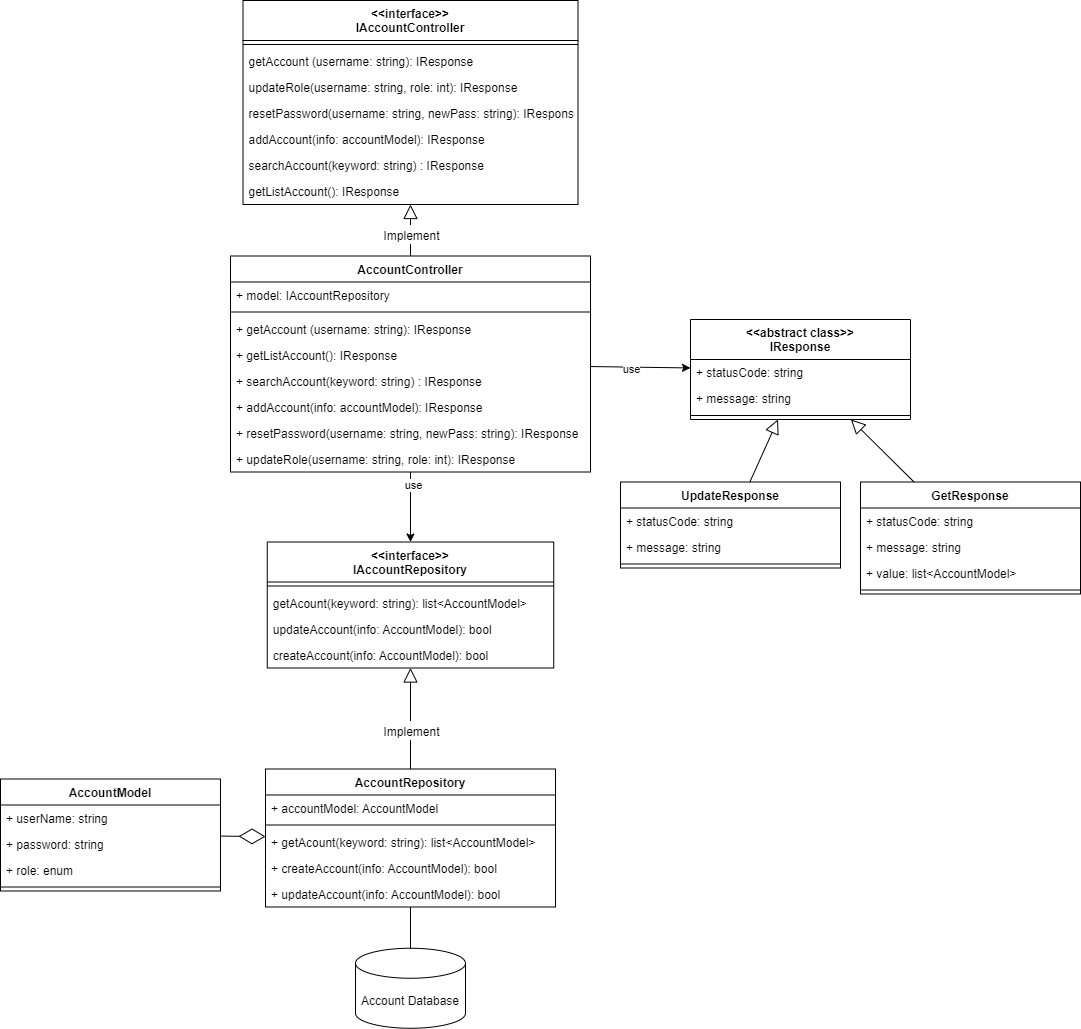
\includegraphics[width=14cm]{img/Architecture/service/AccountService.png}
	\newline
	\caption{Lược đồ class của Account Service}
\end{figure}

\subsubsubsection*{AccountRepository}
Thuộc tính:
\begin{itemize}
	\item accountModel: Chứa đối tượng AccountModel
\end{itemize}
Phương thức:
\begin{itemize}
	\item getAcount(keyword: string): Lấy danh sách tài khoản theo từ khóa
	\item createAccount(info: AccountModel): Tạo một tài khoản mới
	\item updateAccount(info: AccountModel): Cập nhật thông tin một tài khoản
\end{itemize}

\subsubsubsection*{AccountController}
Thuộc tính:
\begin{itemize}
	\item repo: Chứa đối tượng AccountRepository
\end{itemize}
Phương thức:
\begin{itemize}
	\item getAcount(username: string): Lấy tài khoản theo tên đăng nhập
	\item getListAccount(): Lấy danh sách tất cả tài khoản
	\item searchAccount(keyword: string) : Lấy danh sách tài khoản theo từ khóa
	\item addAccount(info: accountModel): Tạo một tài khoản mới
	\item resetPassword(username: string, newPass: string): Tái thiết lập mật khẩu
	\item updateRole(username: string, role: int): Cập nhật quyền tài khoản
\end{itemize}


\subsubsubsection*{UpdateResponse - GetResponse}
Thuộc tính:
\begin{itemize}
	\item statusCode: Mã trạng thái của phản hồi
	\item message: Thông điệp của phản hồi
	\item value: Các dữ liệu trả về đối với các yêu cầu HTTP GET
\end{itemize}

\newpage


\subsubsection{Staff Service}
\begin{figure}[!htp]
	\centering
	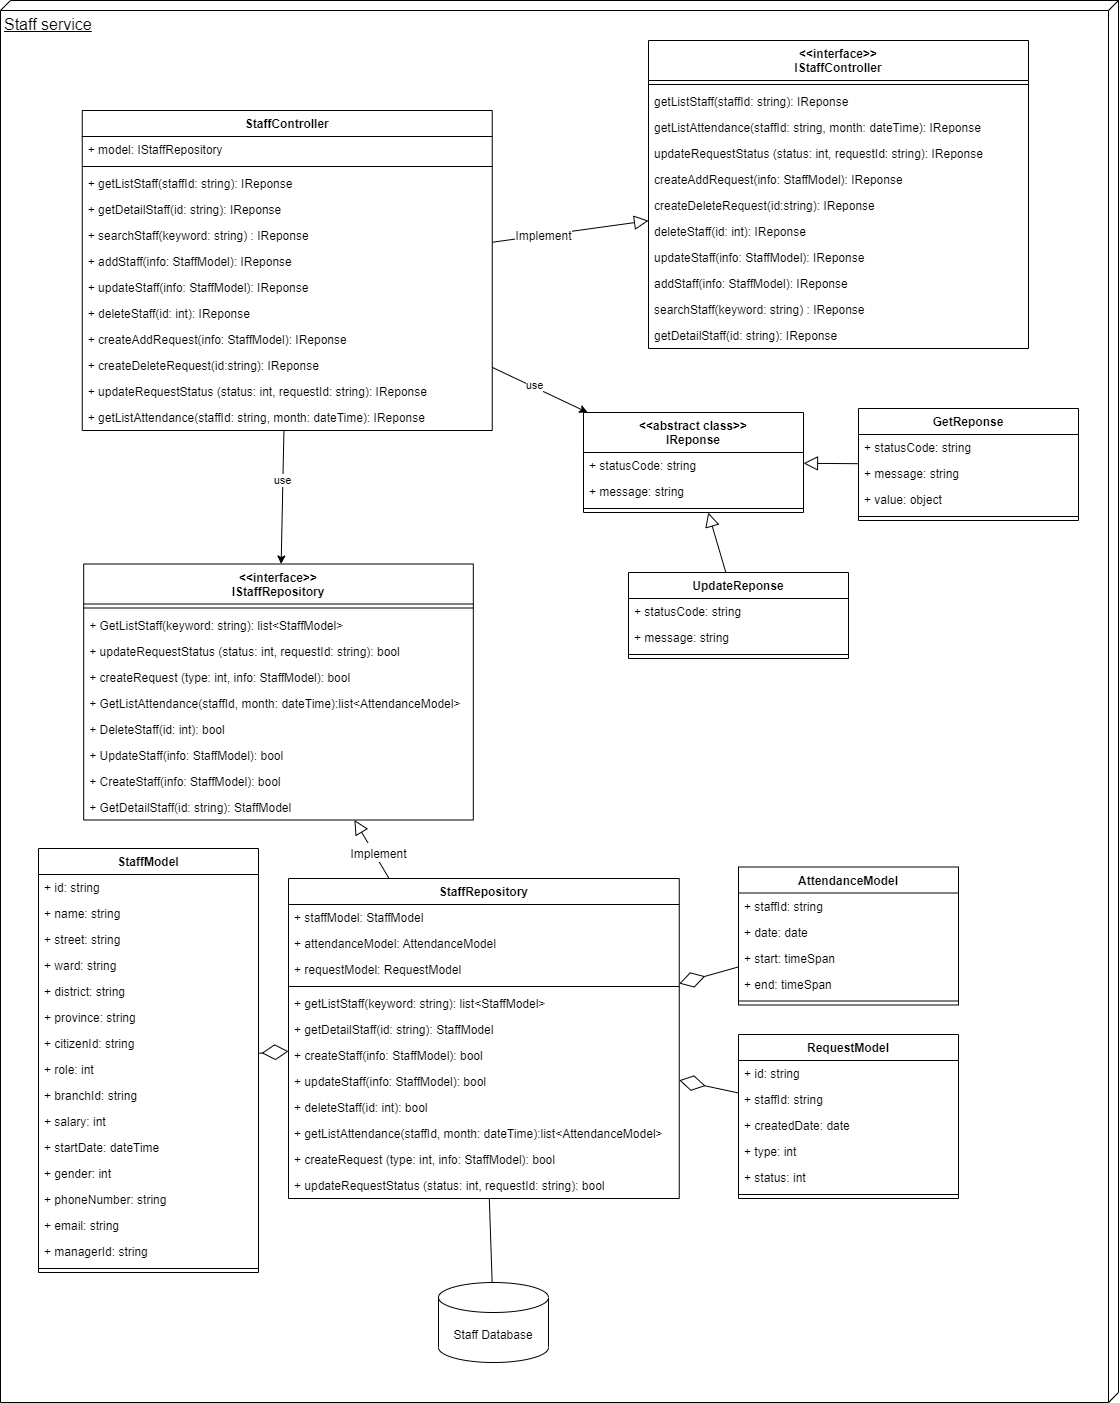
\includegraphics[width=13cm]{img/Architecture/service/StaffService.png}
	\newline
	\caption{Lược đồ class của Staff Service}
\end{figure}

\subsubsubsection*{StaffRepository}
Thuộc tính:
\begin{itemize}
	\item staffModel: Chứa đối tượng StaffModel
	\item attendanceModel: Chứa đối tượng AttendanceModel
	\item requestModel: Chứa đối tượng RequestModel
\end{itemize}
Phương thức:
\begin{itemize}
	\item getListStaff(keyword: string): Lấy danh sách nhân viên theo từ khóa
	\item getDetailStaff(id: string): Lấy thông tin chi tiết một nhân viên
	\item createStaff(info: StaffModel): Thêm một nhân viên mới
	\item updateStaff(info: StaffModel): Cập nhật thông tin một nhân viên
	\item deleteStaff(id: string): Xóa một nhân viên
	\item getListAttendance(staffId, month: dateTime): Lấy danh sách điểm danh của nhân viên
	\item createRequest (type: int, info: StaffModel): Tạo một yêu cầu về thêm, xóa nhân viên
	\item updateRequestStatus (status: int, requestId: string): Cập nhật trạng thái cùa yêu cầu
\end{itemize}

\subsubsubsection*{StaffController}
Thuộc tính:
\begin{itemize}
	\item repo: Chứa đối tượng StaffRepository
\end{itemize}
Phương thức:
\begin{itemize}
	\item getListStaff(branchId: string): Lấy danh sách nhân viên theo chi nhánh
	\item getDetailStaff(id: string): Lấy thông tin chi tiết một nhân viên
	\item searchStaff(keyword: string): Lấy danh sách nhân viên theo từ khóa
	\item createStaff(info: StaffModel): Thêm một nhân viên mới
	\item updateStaff(info: StaffModel): Cập nhật thông tin một nhân viên
	\item deleteStaff(id: string): Xóa một nhân viên
	\item createAddRequest(info: StaffModel): Tạo một yêu cầu thêm nhân viên
	\item createDeleteRequest(id:string): Tạo một yêu cầu về xóa nhân viên
	\item updateRequestStatus (status: int, requestId: string): Cập nhật trạng thái cùa yêu cầu
	\item getListAttendance(staffId, month: dateTime): Lấy danh sách điểm danh của nhân viên
\end{itemize}

\subsubsubsection*{UpdateResponse - GetResponse}
Thuộc tính:
\begin{itemize}
	\item statusCode: Mã trạng thái của phản hồi
	\item message: Thông điệp của phản hồi
	\item value: Các dữ liệu trả về đối với các yêu cầu HTTP GET
\end{itemize}

\newpage


\subsubsection{Branch Service}
\begin{figure}[!htp]
	\centering
	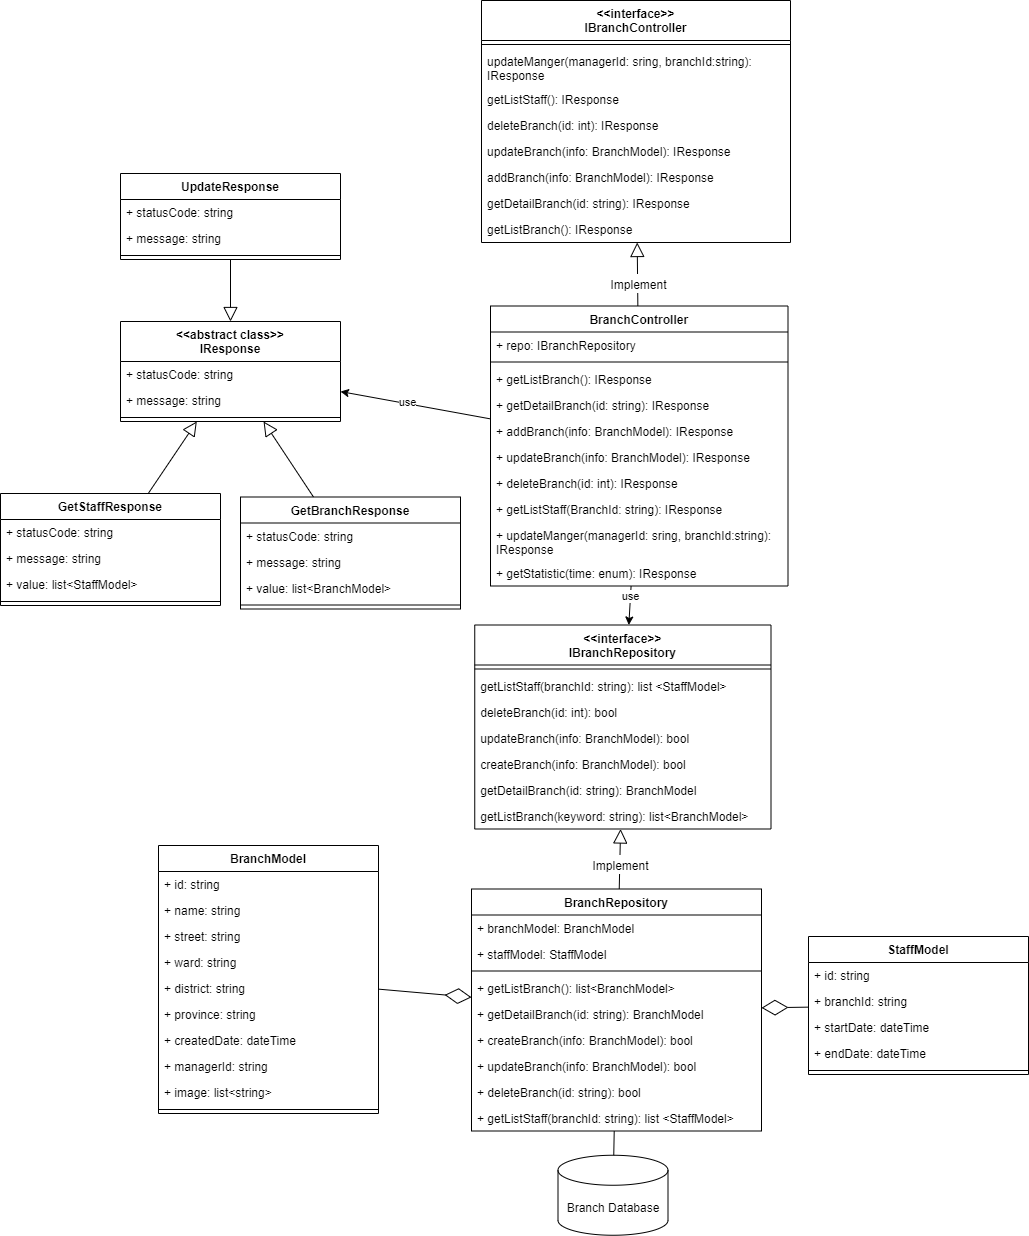
\includegraphics[width=13cm]{img/Architecture/service/BranchService.png}
	\newline
	\caption{Lược đồ class của Branch Service}
\end{figure}

\subsubsubsection*{BranchRepository}
Thuộc tính:
\begin{itemize}
	\item branchModel: Chứa đối tượng BranchModel
	\item staffModel: Chứa đối tượng StaffModel
\end{itemize}
Phương thức:
\begin{itemize}
	\item getListBranch(): Lấy danh sách chi nhánh
	\item getDetailBranch(id: string): Lấy thông tin chi tiết một chi nhánh
	\item createBranch(info: BranchModel): Thêm một chi nhánh mới
	\item updateBranch(info: BranchModel): Cập nhật thông tin một chi nhánh
	\item deleteBranch(id: string): Xóa một chi nhánh
	\item getListStaff(BranchId: string): Lấy danh sách nhân viên của chi nhánh
\end{itemize}

\subsubsubsection*{BranchController}
Thuộc tính:
\begin{itemize}
	\item repo: Chứa đối tượng repository
\end{itemize}
Phương thức:
\begin{itemize}
	\item getListBranch(): Lấy danh sách chi nhánh
	\item getDetailBranch(id: string): Lấy thông tin chi tiết một chi nhánh
	\item addBranch(info: BranchModel): Thêm một chi nhánh mới
	\item updateBranch(info: BranchModel): Cập nhật thông tin một chi nhánh
	\item deleteBranch(id: int): Xóa một chi nhánh
	\item getListStaff(BranchId: string): Lấy danh sách nhân viên của chi nhánh
	\item updateManger(managerId: sring, branchId:string): Cập nhật quản lý chi nhánh
	\item getStatistic(time: enum): Lấy thông tin thống kê lợi nhuận, doanh thu.
\end{itemize}

\subsubsubsection*{UpdateResponse - GetStaffResponse - GetBranchResponse }
Thuộc tính:
\begin{itemize}
	\item statusCode: Mã trạng thái của phản hồi
	\item message: Thông điệp của phản hồi
	\item value: Các dữ liệu trả về đối với các yêu cầu HTTP GET
\end{itemize}

\newpage


\subsubsection{Event Service}
\begin{figure}[!htp]
	\centering
	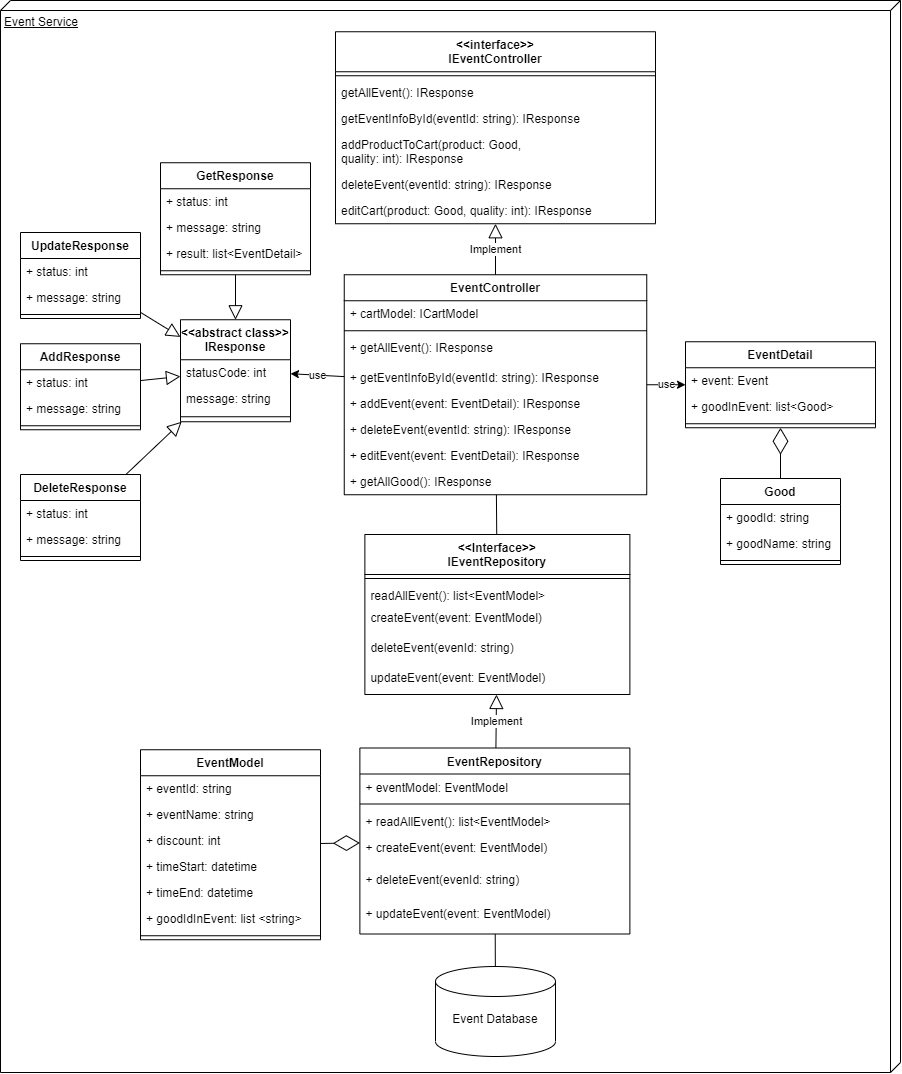
\includegraphics[width=11cm]{img/Architecture/service/EventService.png}
	\newline
	\caption{Lược đồ class của Event Service}
\end{figure}

\subsubsubsection*{EventRepository}
Thuộc tính:
\begin{itemize}
	\item eventModel: Chứa đối tượng EventModel
\end{itemize}
Phương thức:
\begin{itemize}
	\item readAllEvent(): lấy danh sách toàn bộ sự kiện của hệ thống.
	\item readEvent(eventId: string): lấy thông tin chi tiết của sự kiện trong hệ thống.
	\item deleteEvent(eventId: string): xóa sự kiện khỏi hệ thống.g.
	\item createEvent(event: EventModel): tạo sự kiện mới.
	\item updateEvent(event: EventModel): cập nhật thông tin của sự kiện.
\end{itemize}

\subsubsubsection*{EventController}
Thuộc tính:
\begin{itemize}
	\item repo: Chứa đối tượng EventRepository
\end{itemize}
Phương thức:
\begin{itemize}
	\item getAllEvent(): Xử lý dữ liệu và gọi lấy danh sách toàn bộ sự kiện của hệ thống.
	\item getEventInfoById(eventId: string): Xử lý dữ liệu và gọi lấy thông tin chi tiết của sự kiện trong hệ thống.
	\item deleteEvent(eventId: string): Xử lý dữ liệu và gọi xóa sự kiện khỏi hệ thống.
	\item addEvent(event: EventDetail): Xử lý dữ liệu và gọi tạo sự kiện mới.
	\item updateEvent(event: EventDetail): Xử lý dữ liệu và gọi cập nhật thông tin của sự kiện.
	\item getAllGood(): Xử lý dữ liệu và gọi lấy thông tin toàn bộ hàng.
\end{itemize}

\subsubsubsection*{GetResponse - AddResponse - UpdateResponse - DeleteResponse}
Thuộc tính:
\begin{itemize}
	\item statusCode: Mã trạng thái của phản hồi
	\item message: Thông điệp của phản hồi
	\item value: Các dữ liệu trả về đối với các yêu cầu
\end{itemize}

\newpage



\subsubsection{Warehouse Service}
\begin{figure}[!htp]
	\centering
	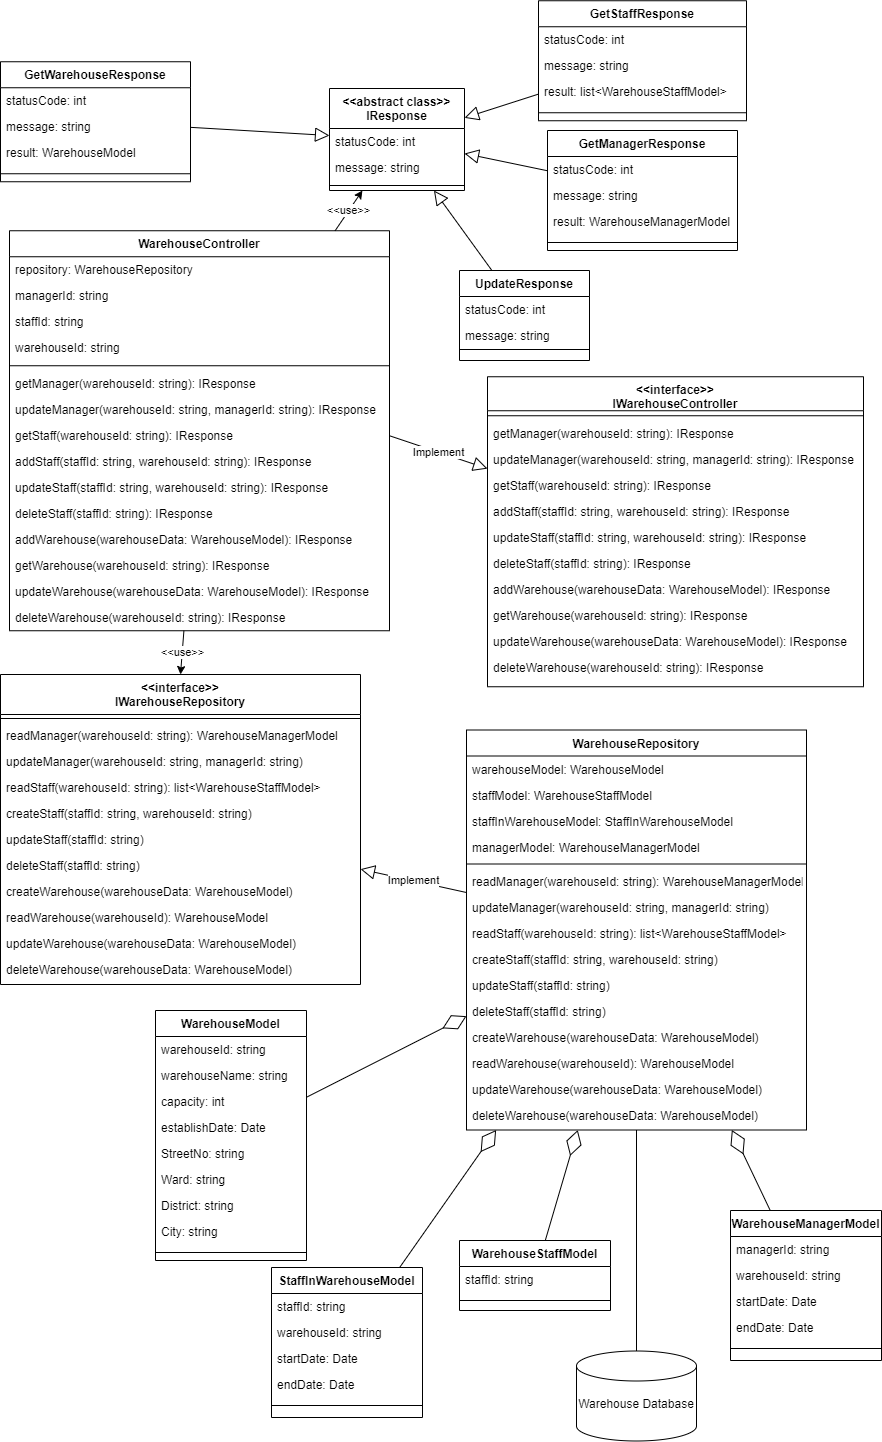
\includegraphics[width=11cm]{img/Architecture/service/WarehouseService.png}
	\newline
	\caption{Lược đồ class của Warehouse Service}
\end{figure}
\subsubsubsection*{WarehouseRepository}
Thuộc tính:
\begin{itemize}
	\item warehouseModel: Chứa đối tượng WarehouseModel
	\item staffModel: Chứa đối tượng WarehouseStaffModel
	\item staffInWarehouseModel: Chứa đối tượng StaffInWarehouseModel
	\item managerModel: Chứa đối tượng ManagerModel
\end{itemize}
Phương thức:
\begin{itemize}
	\item readManager(): Lấy thông tin quản lý kho.
	\item updateManager(): Cập nhật quản lý kho.
	\item readStaff(): Lấy thông tin nhân viên kho.
	\item createStaff(): Thêm nhân viên kho.
	\item updateStaff(): Cập nhật thông tin nhân viên kho.
	\item deleteStaff(): Xóa nhân viên kho.
	\item createWarehouse(): Thêm kho mới.
	\item readWarehouse(): Lấy dữ liệu kho.
	\item updateWarehouse(): Cập nhật dữ liệu kho.
	\item deleteWarehouse(): Xóa kho
\end{itemize}

\subsubsubsection*{WarehouseController}
Phương thức:
\begin{itemize}
	\item getManager(warehouseId: string): Lấy thông tin quản lý kho.
	\item updateManager(warehouseId: string, managerId: string): Cập nhật quản lý cho kho.
	\item getStaff(warehouseId: string): Lấy dữ liệu nhân viên của kho.
	\item addStaff(staffId: string, warehouseId: string): Thêm nhân viên vào kho.
	\item updateStaff(staffId: string, warehouseId: string): Cập nhật thông tin làm việc của nhân viên.
	\item deleteStaff(staffId): Xóa nhân viên.
	\item addWarehouse(warehouseData: WarehouseModel): Thêm kho mới.
	\item getWarehouse(warehouseId): Lấy thông tin kho.
	\item updateWarehouse(warehouseData: WarehouseModel): Cập nhật thông tin kho.
	\item deleteWarehouse(warehouseId: string): Xóa kho.
\end{itemize}

\subsubsubsection*{GetWarehouseResponse - GetStaffResponse - GetManagerResponse - UpdateResponse}
Thuộc tính:
\begin{itemize}
	\item statusCode: Mã trạng thái của phản hồi
	\item message: Thông điệp của phản hồi
	\item value: Các dữ liệu trả về đối với các yêu cầu
\end{itemize}

\newpage



\subsubsection{Statistic Service}
\begin{figure}[!htp]
\centering
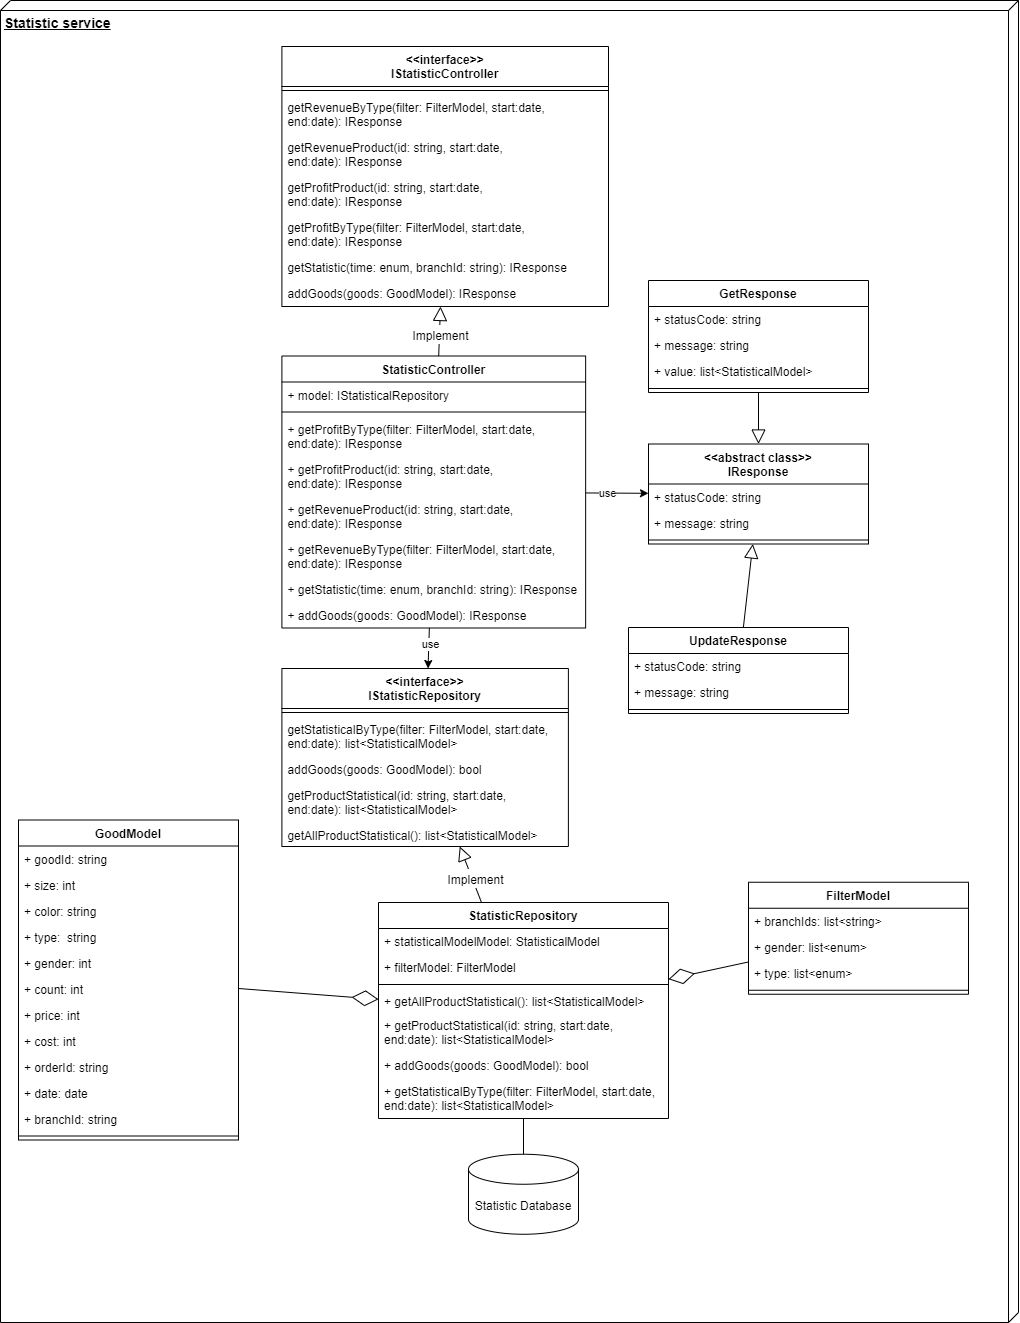
\includegraphics[width=11cm]{img/Architecture/service/StatisticService.png}
\newline
	\caption{Lược đồ class của Statistic Service}
\end{figure}
\subsubsubsection*{StatisticRepository}
Thuộc tính:
\begin{itemize}
	\item statisticalModel: Chứa đối tượng StatisticalModel
	\item filterModel: Chứa đối tượng FilterModel
\end{itemize}
Phương thức:
\begin{itemize}
	\item getAllProductStatistical(): Lấy thông tin thống kê tất cả sản phẩm
	\item getProductStatistical(id: string, start:date,
	      end:date): Lấy thông tin thống kê của một sản phẩm
	\item addGoods(goods: GoodModel): Cập nhật thông tin hàng vào Database
	\item getStatisticalByType(filter: FilterModel, start:date,
	      end:date): Lấy thông tin thống kê các sản phẩm theo bộ lọc
\end{itemize}

\subsubsubsection*{StatisticController}
Thuộc tính:
\begin{itemize}
	\item repo: Chứa đối tượng StatisticRepository
\end{itemize}
Phương thức:
\begin{itemize}
	\item getProfitByType(filter: FilterModel, start:date,
	      end:date): Lấy thông tin lợi nhuận các mặt hàng theo bộ lọc
	\item getProfitProduct(id: string, start:date,
	      end:date): Lấy thông tin lợi nhuận của một sản phẩm
	\item getRevenueProduct(id: string, start:date,
	      end:date): Lấy thông tin doanh thu các mặt hàng theo bộ lọc
	\item getRevenueByType(filter: FilterModel, start:date,
	      end:date): Lấy thông tin doanh thu của một sản phẩm
	\item addGoods(info: BranchModel): Thêm một mặt hàng vào thống kê
\end{itemize}

\subsubsubsection*{UpdateResponse - GetResponse}
Thuộc tính:
\begin{itemize}
	\item Tầng User Interface: Tầng giao diện tương tác với người dùng
	\item Tầng BPEL: Tầng xây dựng quy trình BPEL, điều phối các quy trình nghiệp vụ trong hệ thống
	\item Tầng API Gateway: Tầng xuất các Api từ các dịch vụ web đưa đến quy trình BPEL
	\item Tầng BFF: Đóng vai trò trong việc kiểm tra các hoạt động trung gian khi nhận yêu cầu từ phía người dùng
	\item Tầng Web Service: Bao gồm các dịch vụ Web
\end{itemize}
\newpage



\subsubsection{Goods Service}
\begin{figure}[!htp]
	\centering
	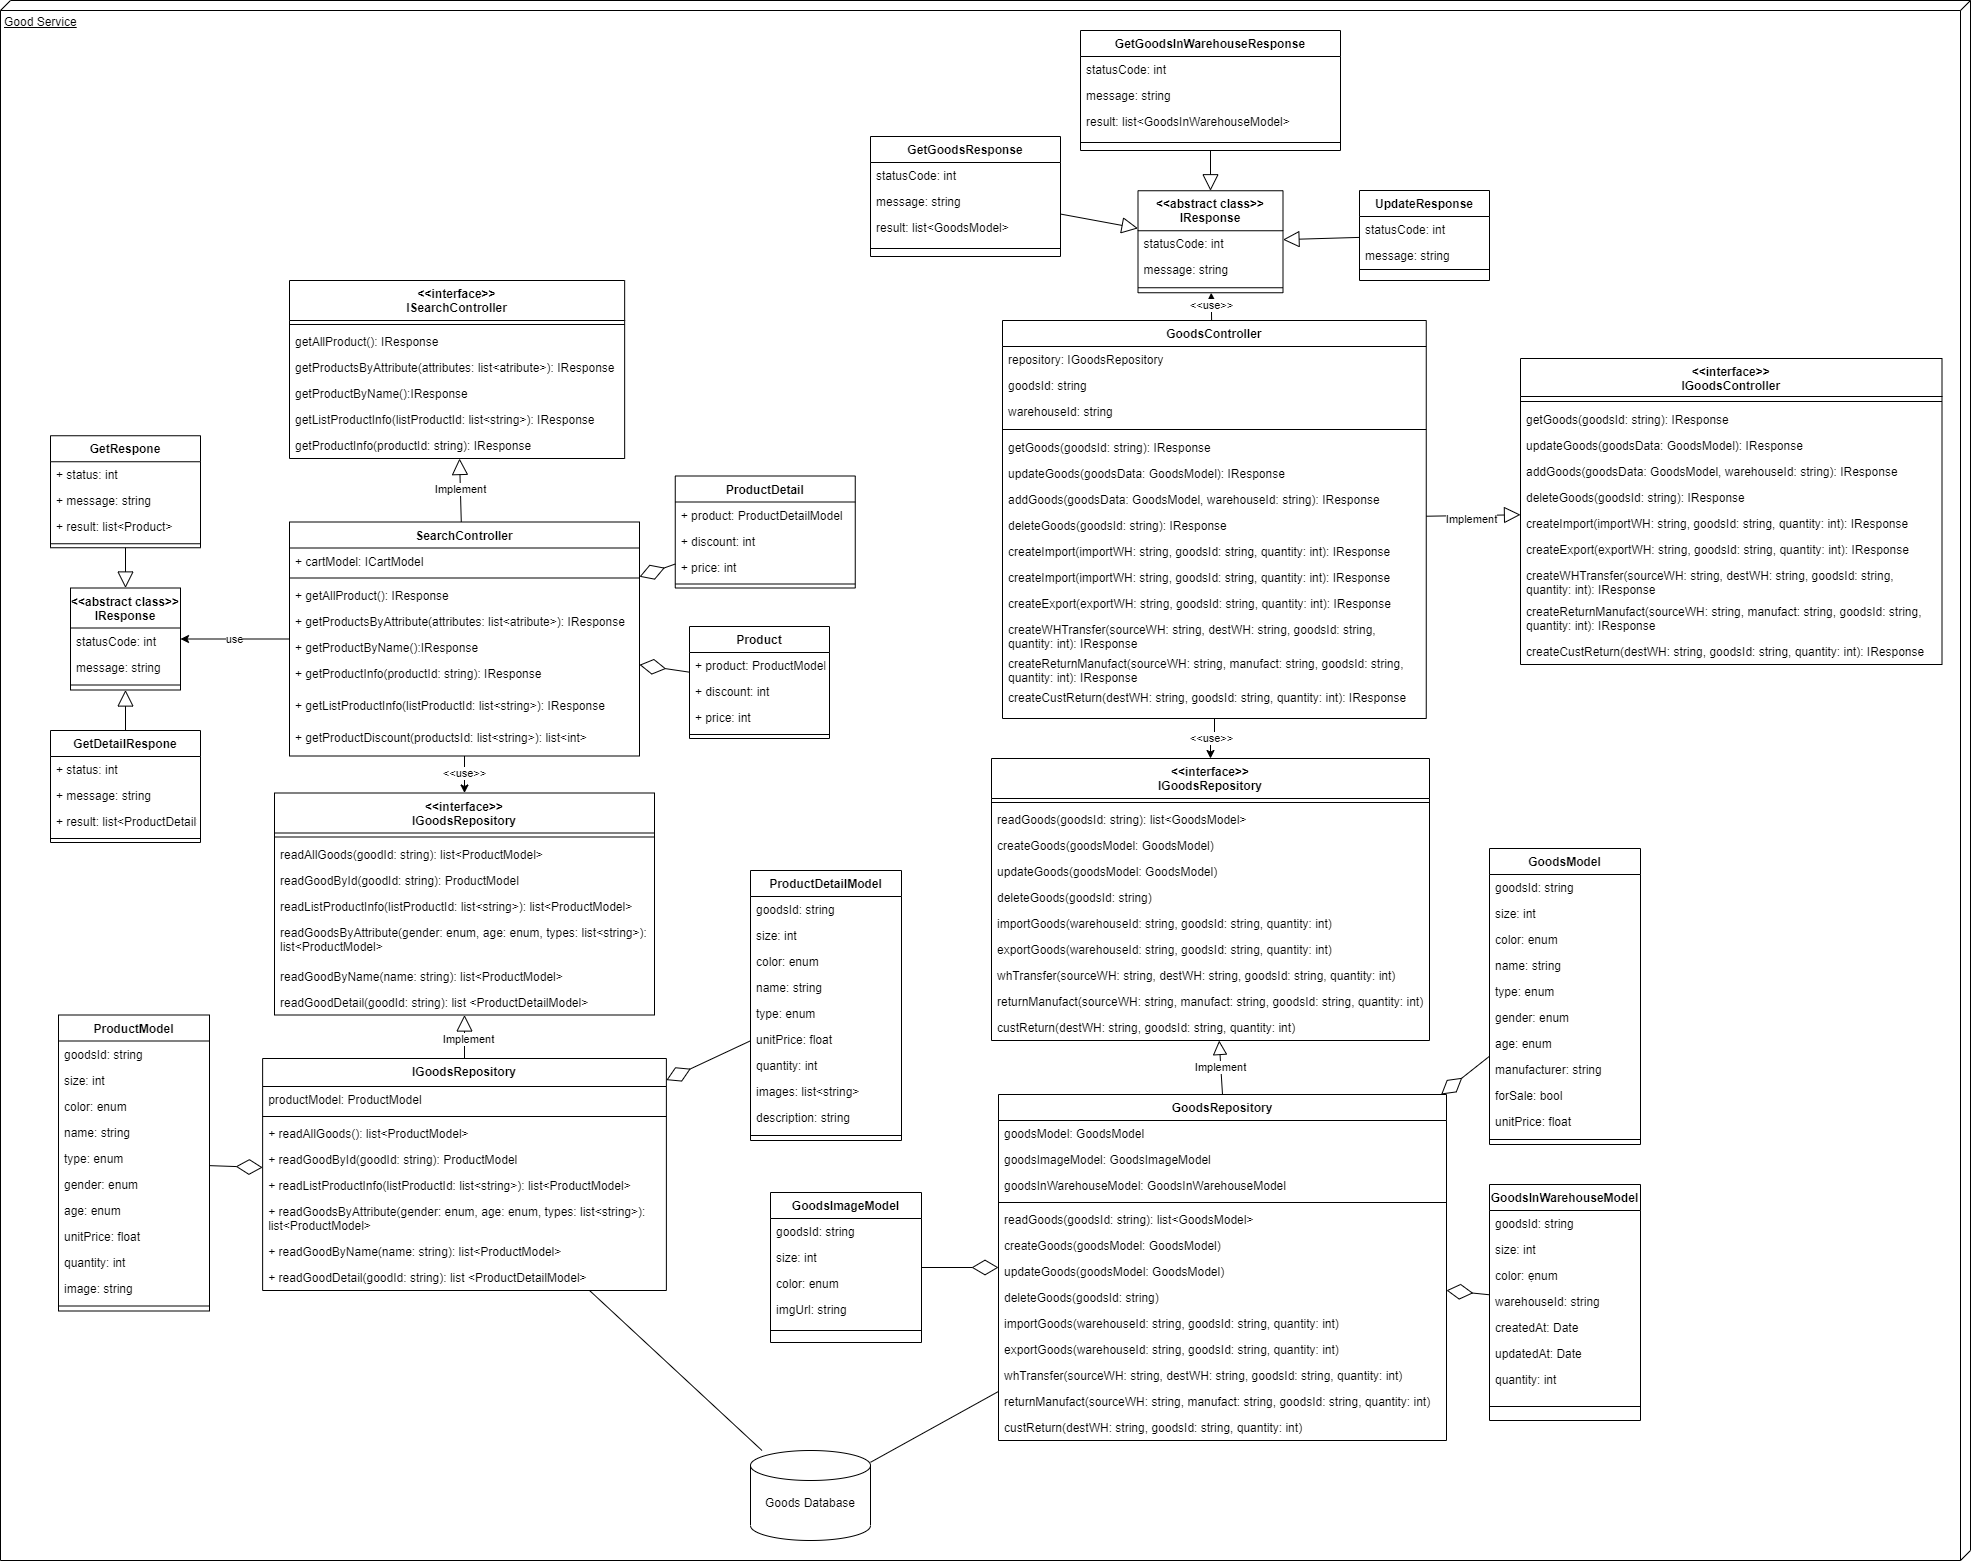
\includegraphics[width=17.5cm]{img/Architecture/service/GoodsService.png}
	\newline
	\caption{Lược đồ class của Goods Service}
\end{figure}
\subsubsubsection*{GoodsRepository}
Thuộc tính:
\begin{itemize}
	\item goodsModel: Chứa đối tượng GoodsModel
	\item goodsImageModel: Chứa đối tượng GoodsImageModel
	\item goodsInWarehouseModel: Chứa đối tượng GoodsInWarehouseModel
\end{itemize}
Phương thức:
\begin{itemize}
	\item readGoods(): Lấy thông tin hàng.
	\item updateGoods(): Cập nhật thông tin hàng.
	\item createGoods(): Thêm hàng.
	\item deleteGoods(): Xóa hàng.
	\item importGoods(): Nhập hàng.
	\item exportGoods(): Xuất hàng.
	\item whTransfer(): Luân chuyển hàng.
	\item returnManufact(): Trả hàng về nhà cung cấp.
	\item custReturn(): Người dùng trả hàng.
\end{itemize}

\subsubsubsection*{GoodsController}
Thuộc tính:
\begin{itemize}
	\item repository: chứa đối tượng IGoodsRepository.
	\item goodsId: mã hàng.
	\item warehouseId: mã kho.
\end{itemize}
Phương thức:
\begin{itemize}
	\item getGoods(goodsId: string): Lấy thông tin hàng.
	\item updateGoods(goodsData: GoodsModel): Cập nhật thông tin hàng.
	\item addGoods(goodsData: GoodsModel, warehouseId: string): Tạo hàng và thêm vào kho.
	\item deleteGoods(goodsId: string): Xóa hàng.
	\item createImport(importWH: string, goodsId: string, quantity: int): Tạo yêu cầu nhập kho.
	\item createExport(exportWH: string, goodsId: string, quantity: int): Tạo yêu cầu xuất kho.
	\item createWHTransfer(sourceWH: string, destWH: string, goodsId: string, quantity: int): Tạo yêu cầu luân chuyển hàng.
	\item createReturnManufact(sourceWH: string, manufact: string, goodsId: string, quantity: int): Tạo yêu cầu trả hàng về nhà cung cấp.
	\item createCustReturn(destWH: string, goodsId: string, quantity: int): Tạo dữ liệu người dùng trả hàng.
\end{itemize}

\subsubsubsection*{GetGoodsResponse - GetGoodsInWarehouseResponse - UpdateResponse}
Thuộc tính:
\begin{itemize}
	\item statusCode: Mã trạng thái của phản hồi
	\item message: Thông điệp của phản hồi
	\item result: Các dữ liệu trả về đối với các yêu cầu
\end{itemize}


\newpage



\subsubsection{Giao tiếp đồng bộ giữa các Services}

\hspace*{0.5cm} Để hiện thực việc giao tiếp đồng bộ giữa các service, chúng ta có hai cách tiếp cận là giao tiếp thông qua bộ điều phối trung tâm (Orchestration) và giao tiếp trực tiếp giữa các service (Choreography). Với cách tiếp cận Choreography, các service sẽ gọi trực tiếp với nhau tùy theo mục đích của mình. Còn với cách tiếp cận Orchestration, một service trung gian sẽ được tạo ra để phục vụ cho việc giao tiếp giữa các service trong hệ thống; mục đích của service này là để quản lý và điều phối các lần gọi nhau giữa các service. 
\par Ví dụ, với hệ thống có hai service Customer Wishlist và Customer Demographics. Service Customer Wishlist được dùng để quản lý danh sách yêu thích của người dùng, còn service Customer Demographics được dùng để quản lý thông tin người dùng. Hiện tại, người dùng 123 có nhu cầu lấy thông tin chi tiết về danh sách yêu thích của mình. Do service Customer Wishlist chưa lưu tất cả các thông tin cần thiết, nên nó cần gọi service Customer Demographics để lấy thêm dữ liệu.

\par Nếu sử dụng Choreography, sơ đồ giao tiếp giữa các service được trình bày như sau:
\begin{figure}[!htp]
	\centering
	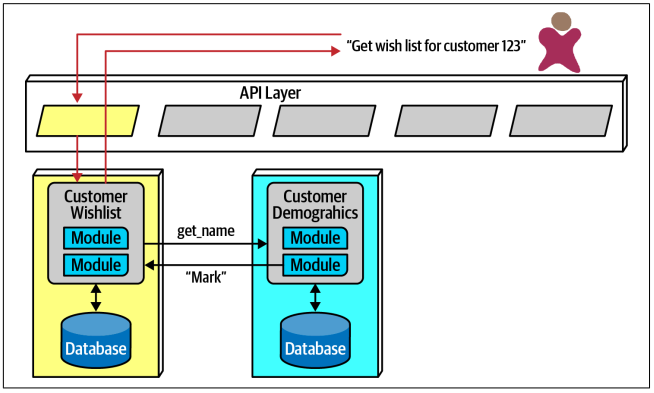
\includegraphics[width=8cm]{img/Architecture/choreography.PNG}
	\newline
	\caption{Giao tiếp giữa các service bằng Choreography \cite{archChoreography}}
\end{figure}

Đối với phương pháp giao tiếp Choreography, service Customer Wishlist gọi trực tiếp đến service Customer Demographics để lấy thông tin từ user mà không đi qua trung gian nào cả. Và service Customer Demographics cũng trả về kết quả trực tiếp cho service Customer Wishlist.

\par Nếu sử dụng Orchestration, sơ đồ giao tiếp giữa các service được trình bày như sau:

\begin{figure}[!htp]
	\centering
	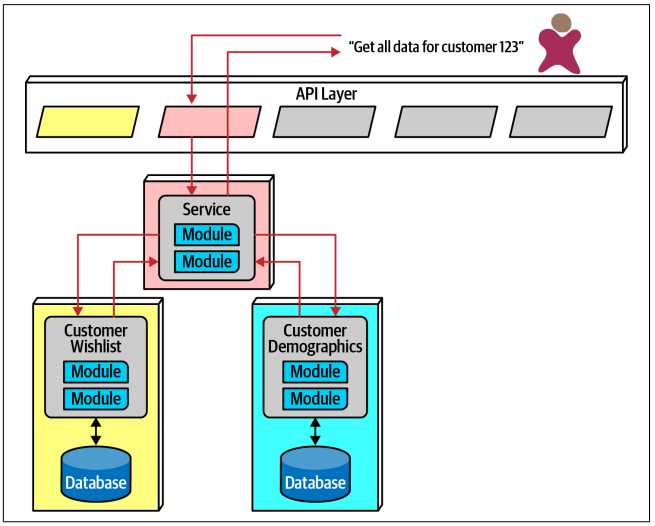
\includegraphics[width=8cm]{img/Architecture/orchestration.PNG}
	\newline
	\caption{Giao tiếp giữa các service bằng Orchestration \cite{archOrchestration}}
\end{figure}
Đối với phương pháp giao tiếp Orchestration, một service trung gian được tạo ra, với vai trò điều phối việc gọi nhau để lấy thông tin giữa service Customer Wishlist và Customer Demographics. Khi nhận được yêu cầu lấy thông tin từ người dùng, service trung gian gọi đến các service đích để lấy thông tin: gọi đến Customer Wishlist để lấy thông tin danh sách yêu thích, và gọi đến Customer Demographics để lấy thông tin người dùng.

\par Mỗi phương pháp có các ưu điểm và nhược điểm riêng. Đối với Choreography, cách tiếp cận này giúp giảm đi tính phụ thuộc giữa các service (decoupled), và đây cũng là mục đích đối với hệ thống microservice. Tuy vậy, việc quản lý lỗi và quản lý luồng thực thi sẽ là vấn đề lớn ở phương pháp này. Còn đối với Orchestration, đây là phương pháp hợp lý cho các công việc có luồng nghiệp vụ phức tạp, tuy vậy sẽ tạo nên sự phụ thuộc lẫn nhau giữa các service.

\par Ở hệ thống này, nhóm lựa chọn phương pháp Choreography để hiện thực việc giao tiếp giữa các service, để đảm bảo tính phân chia rõ ràng và ít phụ thuộc (loosely-coupled) giữa các service, đồng thời hạn chế các nhược điểm khi luồng thực thi trong những lần gọi là không phức tạp.

\subsubsubsection{Giao tiếp của Customer order Service}
\begin{figure}[!htp]
	\centering
	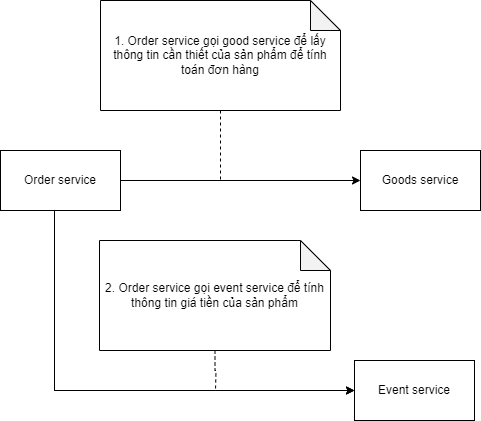
\includegraphics[width=8cm]{img/Architecture/service/customer-order-call.png}
	\newline
	\caption{Lược đồ giao tiếp đồng bộ của Customer order Service với các dịch vụ khác}
\end{figure}

\begin{itemize}
	\item \textbf{Goods service}: Customer order service gọi tới Goods service để thực hiện lấy thông tin cần thiết của sản phẩm, sử dụng dữ liệu đó để tính toán cho đơn hàng cũng như tạo đơn hàng.
	\item \textbf{Event service}: Customer order service gọi tới Event service để thực hiện lấy thông tin sự kiện giảm giá để tính toán giá tiền cho đơn hàng.
	\item \textbf{Customer service}: Customer order service gọi tới Customer service để thực hiện lấy thông tin người dùng để tạo đơn hàng và tự đồng điền form.
	\item \textbf{Transport service}: Customer order service gọi tới Transport service để thực hiện lấy thông tin giá tiền vận chuyển.
	\item \textbf{Payment service}: Customer order service gọi tới Payment service để thực hiện thanh toán trực tuyến khi người dùng chọn phương thức thanh toán trực tuyến tương ứng.
\end{itemize}


\subsubsubsection{Giao tiếp của Cart Service}
\begin{figure}[!htp]
	\centering
	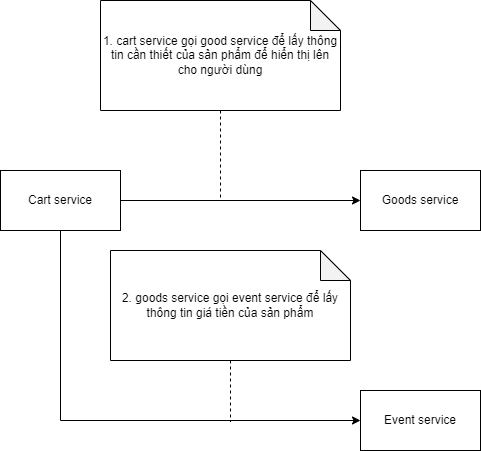
\includegraphics[width=8cm]{img/Architecture/service/cart-call.png}
	\newline
	\caption{Lược đồ giao tiếp đồng bộ của Cart Service với các dịch vụ khác}
\end{figure}

\begin{itemize}
	\item \textbf{Goods service}: Cart service gọi tới Goods service để thực hiện lấy thông tin cần thiết của sản phẩm, sử dụng dữ liệu đó để tính toán cho tổng giá tiền trong giỏ hàng.
	\item \textbf{Event service}: Cart service gọi tới Event service để thực hiện lấy thông tin sự kiện giảm giá để tính toán giá tiền cho sản phẩm trong giỏ hàng.
\end{itemize}

\newpage
\subsubsubsection{Giao tiếp của Staff Service}
\begin{figure}[!htp]
	\centering
	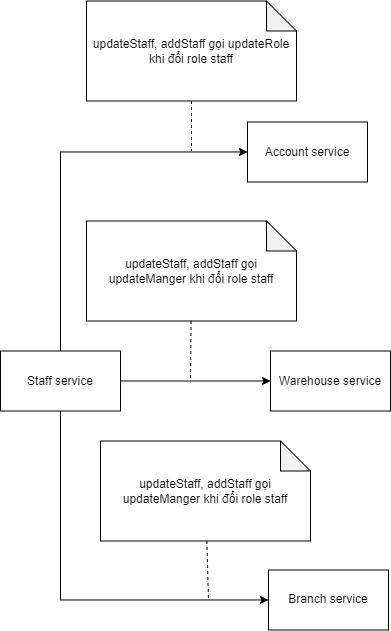
\includegraphics[width=7cm]{img/Architecture/service/staff-call.png}
	\newline
	\caption{Lược đồ giao tiếp đồng bộ của Staff Service với các dịch vụ khác}
\end{figure}

\begin{itemize}
	\item \textbf{Account service}: Staff service gọi tới Account service để thực hiện cập nhật hoặc thêm tài khoản của nhân viên.
	\item \textbf{Warehouse service}: Staff service gọi tới Warehouse service để thực hiện cập nhật lại thông tin quản lý khi đổi quyền của nhân viên.
	\item \textbf{Branch service}: Staff service gọi tới Branch service để thực hiện cập nhật lại thông tin quản lý khi đổi quyền của nhân viên.
\end{itemize}

\subsubsubsection{Giao tiếp của Account Service}
\begin{figure}[!htp]
	\centering
	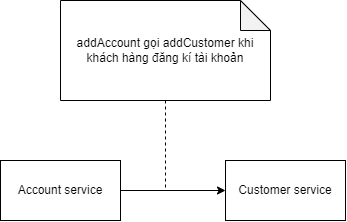
\includegraphics[width=6cm]{img/Architecture/service/account-call.png}
	\newline
	\caption{Lược đồ giao tiếp đồng bộ của Account Service với các dịch vụ khác}
\end{figure}

\begin{itemize}
	\item \textbf{Customer service}: Account service gọi tới Customer service để thực hiện thêm người dùng tương ứng với tài khoản vừa được tạo.
\end{itemize}

\subsubsection{Giao tiếp bất đồng bộ giữa các Services}
 
 
\hspace*{0.5cm} Giao tiếp bất đồng bộ diễn ra ở các tác vụ không yêu cầu phản hồi kết quả ngay, thay vào đó yêu cầu gọi sẽ được lưu lại và xử lý sau. Việc giao tiếp bất đồng bộ giảm việc sử dụng tài nguyên của hệ thống, trong khi vẫn đảm bảo được kết quả trả về.
 
\par Khi phía client gửi một yêu cầu (request) đến phía server, client sẽ chờ server xử lý xong toàn bộ quá trình theo quy trình nghiệp vụ rồi mới kết thúc.
Đối với các tác vụ lớn hoặc yêu cầu thời gian xử lý lớn, phía client sẽ phải chờ lâu, và điều này làm hao phí tài nguyên của hệ thống. Bằng việc áp dụng giao tiếp bất đồng bộ vào các tác vụ thích hợp, hệ thống sẽ giảm được việc sử dụng tài nguyên hệ thống khi client phải phản hồi lâu từ server.
Các request trước khi được xử lý bằng giao tiếp bất đồng bộ sẽ được kiểm tra kĩ về mặt dữ liệu, để đảm bảo các lỗi liên quan đến dữ liệu request sẽ không xuất hiện khi xử lý sau. Sau khi xử lý request, kết quả sẽ được gửi về cho phía client.
Phía server sau khi hoàn thành bước kiểm tra dữ liệu và xử lý các tác vụ đồng bộ, sẽ gửi thông điệp vào message queue để gửi đến dịch vụ web đích. Khi việc thêm thông điệp vào message queue thành công, phía server sẽ trả về thành công cho phía client, không cần phía client phải chờ toàn bộ quy trình nghiệp vụ phải xử lý xong.\\
 
Dưới đây là các giao tiếp bất đồng bộ có trong hệ thống:
 
\begin{figure}[!htp]
    \centering
    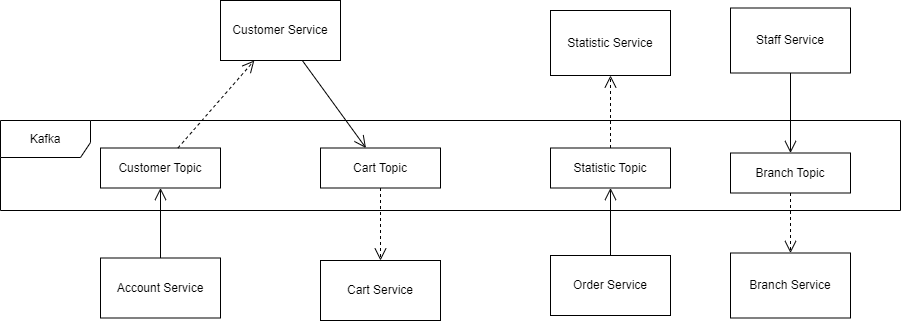
\includegraphics[width=13cm]{img/Architecture/kafka.png}
    \newline
    \caption{Giao tiếp bất đồng bộ giữa các services}
\end{figure}
 
\begin{itemize}
    \item Customer Topic: Customer Service khi thêm một khách hàng mới sẽ gửi dữ liệu đến để Cart Service cập nhật thêm giỏ hàng tương ứng
    \item MakeOrder Topic: Customer Order Service khi nhận được thông tin đơn hàng mới sẽ gửi dữ liệu cập nhật thông tin đơn hàng đó cho Order Service
    \item Statistic Topic: Khi Order Service đã cập nhật thông tin đơn hàng mới sẽ gửi thông tin đơn hàng cho Statistic Service để thống kê
\end{itemize}